% !TEX root = main.tex


% 文章的主体架构章节数均在此设计编辑。


\documentclass[UTF8,twoside,zihao=-4,AutoFakeBold,scheme=chinese,openany]{ctexbook}
\usepackage{graphicx}
% 输入配置文件,例如调用的宏包(公式,插图等)

%设置文章格式

\usepackage[final]{pdfpages}

\usepackage{geometry}
\usepackage{makecell}
\usepackage{caption}
\usepackage{multirow}
\usepackage{booktabs}
\makeatletter
\let\c@lofdepth\relax
\let\c@lotdepth\relax
\makeatother
\usepackage{subfigure}
\usepackage{float}
\usepackage[titles,subfigure]{tocloft}
\usepackage{soul}
\usepackage{color,xcolor}
\usepackage{setspace}
\usepackage{titletoc}
\usepackage{longtable}

\usepackage[list=off]{bicaption}
\usepackage[hidelinks]{hyperref}
%\usepackage{mathptmx} %设置数学公式为新罗马字体
\usepackage{amsmath} %几个数学宏包
\usepackage{fontspec}
%\usepackage{mathspec}
%\usepackage[no-math]{fontspec}
\usepackage{newtxmath}
\usepackage{bm}
%\usepackage{newtxtext}
%\usepackage{unicode-math}
%\usepackage{txfonts}
\usepackage{diagbox}


\AtBeginDocument{\DeclareMathAlphabet{\mathbf}{OT1}{cmr}{bx}{n}}







% 设置页边距
\geometry{a4paper,top=3cm,bottom=3cm,left=3cm,right=3cm}

% 设置行间距 1.5倍
%\linespread{1.4}\selectfont

% 设置段与段之间的垂直距离 \parskip默认橡皮长度是0pt plus 1pt
\setlength{\parskip}{0pt}
%\setlength{\baselineskip}{20pt}
% \setlength{\parindent}{0pt}

% 行间距={}*字体里面的第二个{},对于xiaosi而言就是1等于20磅
\linespread{1}\selectfont

%设置字体
% 设置英文字体
\setmainfont{Times New Roman}[
    BoldFont = Times New Roman Bold,
    ItalicFont = Times New Roman Italic,
    BoldItalicFont = Times New Roman Bold Italic
]

\setsansfont{Times New Roman}[
    BoldFont = Times New Roman Bold,
    ItalicFont = Times New Roman Italic,
    BoldItalicFont = Times New Roman Bold Italic
]

\setmonofont{Times New Roman}[
    BoldFont = Times New Roman Bold,
    ItalicFont = Times New Roman Italic,
    BoldItalicFont = Times New Roman Bold Italic
]

%设置字号,举例\xiaosi表示的是20磅行距,\xiaosid对应的是单倍行距


\usepackage{ctexsize,type1cm}
\newcommand{\chuhaod}{\fontsize{42pt}{54.6pt}\selectfont}
\newcommand{\xiaochud}{\fontsize{36pt}{46.8pt}\selectfont}
%\newcommand{\yihao}{\fontsize{26pt}{39pt}\selectfont}
%\newcommand{\xiaoyi}{\fontsize{24pt}{36pt}\selectfont}   
\newcommand{\erhaod}{\fontsize{22pt}{28.6pt}\selectfont}          
\newcommand{\xiaoerd}{\fontsize{18pt}{23.4pt}\selectfont}          
\newcommand{\sanhaod}{\fontsize{16pt}{20.8pt}\selectfont}        
\newcommand{\xiaosand}{\fontsize{15pt}{19.5pt}\selectfont}        
\newcommand{\sihaod}{\fontsize{14pt}{18.2pt}\selectfont}            
\newcommand{\xiaosid}{\fontsize{12pt}{15.6pt}\selectfont}            
\newcommand{\wuhaod}{\fontsize{10.5pt}{13.65pt}\selectfont}
%\newcommand{\xiaowu}{\fontsize{9pt}{13.5pt}\selectfont}    
%\newcommand{\liuhao}{\fontsize{7.5pt}{11.25pt}\selectfont}

\newcommand{\wuhaob}{\fontsize{10.5pt}{17pt}\selectfont}

\newcommand{\chuhao}{\fontsize{42pt}{42pt}\selectfont}
\newcommand{\xiaochu}{\fontsize{36pt}{36pt}\selectfont}
\newcommand{\yihao}{\fontsize{26pt}{39pt}\selectfont}
\newcommand{\xiaoyi}{\fontsize{24pt}{36pt}\selectfont}   
%\newcommand{\erhao}{\fontsize{22pt}{33pt}\selectfont}          
\newcommand{\xiaoer}{\fontsize{18pt}{27pt}\selectfont}          
\newcommand{\sanhao}{\fontsize{16pt}{20pt}\selectfont}        
\newcommand{\xiaosan}{\fontsize{15pt}{20pt}\selectfont}        
\newcommand{\sihao}{\fontsize{14pt}{20pt}\selectfont}            
\newcommand{\xiaosi}{\fontsize{12pt}{20pt}\selectfont}            
\newcommand{\wuhao}{\fontsize{10.5pt}{20pt}\selectfont}
\newcommand{\xiaowu}{\fontsize{9pt}{13.5pt}\selectfont}    
\newcommand{\liuhao}{\fontsize{7.5pt}{11.25pt}\selectfont}

%使用公式,表格,图片
\usepackage{mathtools,amsmath,amssymb,graphicx,array,float}

%按照章节编号
\numberwithin{figure}{chapter}
\numberwithin{table}{chapter}
\numberwithin{equation}{chapter}

%图、表、公式格式改为 X-X
\renewcommand\thefigure{\arabic{chapter}-\arabic{figure}}
\captionsetup[figure]{labelsep=space}

\renewcommand\thetable{\arabic{chapter}-\arabic{table}}
\captionsetup[table]{labelsep=space}

\renewcommand\theequation{\arabic{chapter}-\arabic{equation}}

%设置图表英文标题格式
\captionsetup{font={stretch=1.2}} %调整中英文图表标题的行距
\setlength{\abovecaptionskip}{6pt} %调整图表标题与图片和表格之间的距离
%\setlength{\belowcaptionskip}{1pt} 
\captionsetup[figure][bi-second]{name=\wuhao Fig.}
\captionsetup[table][bi-second]{name=\wuhao Table}
%\setlength{\captionwidth}{10cm} 




% 设置页眉面脚
%% 设置章节前的页码格式
%\usepackage[pagestyles]{titlesec}
%\newpagestyle{MyStyle}{
%  \setfoot{}{\Roman{page}}{}
%%  \headrule
%}

\usepackage{fancyhdr}

%\fancypagestyle{abstract}
%{
%	\fancyhf{}
%	\renewcommand{\headrulewidth}{0.5pt}
%	%	\renewcommand{\footrulewidth}{0mm}
%	\fancyfoot[C]{\songti\xiaowu \Roman{page}}
%	\fancyhead[C]{\wuhao \leftmark}
%}

%重新设置plain,chapter设置页眉时会调用plain,因此需要重新定义plain,不能设置为其他名称



\fancypagestyle{plain}{
	\fancyhf{}
	\fancyfoot[C]{\songti\xiaowu  \Roman{page} }
	\fancyhead[C]{\songti\wuhao \leftmark}
}





%页眉设置,博士和硕士学位论文请在下面自行修改
\fancypagestyle{body}{
    \fancyhf{}
    \fancyfoot[C]{\songti\xiaowu \thepage}
    \fancyhead[CO]{\songti\wuhao \rightmark}
    \fancyhead[CE]{\songti\wuhao 重庆邮电大学博士学位论文}
}

\fancypagestyle{others}{
	\fancyhf{}
	\fancyfoot[C]{\songti\xiaowu \thepage}
	\fancyhead[CO]{\songti\wuhao \leftmark}
	\fancyhead[CE]{\songti\wuhao 重庆邮电大学博士学位论文}
}







%设置双线页眉
%\makeatletter
%\def\headrule{
%    {\if@fancyplain\let\headrulewidth\plainheadrulewidth\fi%
%    \hrule\@height 1.0pt \@width\headwidth\vskip1pt%上面线为1pt粗
%    \hrule\@height 0pt \@width\headwidth  %下面0.5pt粗
%    \vskip-2\headrulewidth\vskip-1.2pt}    %两条线的距离1pt
%    \vspace{6mm}}     %双线与下面正文之间的垂直间距
%\makeatother

%设置双线页脚
\makeatletter
\def\footrule{
    {\if@fancyplain\let\footrulewidth\plainfootrulewidth\fi%
    \hrule\@height 0pt \@width\headwidth          %上面0.5pt粗
    \vskip 1pt
    \hrule\@height 0pt \@width\headwidth %下面线为1pt粗
    \vskip-2\headrulewidth\vskip-1.2pt}    %两条线的距离1pt
    \vspace{8mm}}     %双线与下面正文之间的垂直间距
\makeatother

%\renewcommand\thechapter{\arabic{chapter}}

%设置文章格式
\ctexset {
    contentsname={目 \quad 录},
    listfigurename={图目录},
    listtablename={表目录},
    figurename={\wuhao 图},
    tablename={\wuhao 表},
    bibname={参考文献},
    appendixname={附录},
    chapter={
    	name={第,章},
    	aftername=\enspace,
    	number={\arabic{chapter}},
        beforeskip={-2pt},
        afterskip={18pt},
        nameformat={\heiti\sanhao\centering\mdseries}, 
        titleformat={\heiti\sanhao\centering\mdseries},
    },
    section={
    	aftername=\enspace,
    	beforeskip={18pt},
    	afterskip={6pt},
        format={\heiti\sihao\leftline},
    },
    subsection={
    	aftername=\enspace,
    	beforeskip={12pt},
    	afterskip={6pt},
        format={\heiti\sihao\leftline},
    },
    subsubsection={
    	aftername=\enspace,
    	beforeskip={12pt},
    	afterskip={6pt},
        format={\heiti\xiaosi\leftline},
    }
}



% 目录中的章加点
%\usepackage[titles]{tocloft}
%\renewcommand{\cftdot}{$\cdot$}
%\renewcommand{\cftdotsep}{1.5}
%\setlength{\cftbeforechapskip}{10pt}
%
%\renewcommand{\cftchapleader}{\cftdotfill{\cftchapdotsep}}
%\renewcommand{\cftchapdotsep}{\cftdotsep}
%\makeatletter
%\renewcommand{\numberline}[1]{
%\settowidth\@tempdimb{#1\hspace{0.5em}}
%\ifdim\@tempdima<\@tempdimb
%  \@tempdima=\@tempdimb
%\fi
%\hb@xt@\@tempdima{\@cftbsnum #1\@cftasnum\hfil}\@cftasnumb}
%\makeatother

% 设置目录字体尺寸
%\renewcommand{\cftchapfont}{\heiti\xiaosi}
%\renewcommand{\cftsecfont}{\heiti\xiaosi}
%\renewcommand{\cftsubsecfont}{\songti\xiaosi}
%\renewcommand{\cftsubsubsecfont}{\songti\xiaosi}

% 设置目录标题深度
\setcounter{secnumdepth}{3}
\setcounter{tocdepth}{2}


% 设置目录标题缩进,字体等
\titlecontents{chapter}[3.8em]{\heiti\xiaosi}{\contentslabel{3.8em}}{\hspace{-3.76em}}{\titlerule*[0.4pc]{$\cdot$}\contentspage\hspace*{0.01em}}
\titlecontents{section}[3.8em]{\songti\xiaosi}{\contentslabel{2em}}{\hspace{-2em}}{\titlerule*[0.4pc]{$\cdot$}\contentspage\hspace*{0.01em}}
\titlecontents{subsection}[6.5em]{\songti\xiaosi}{\contentslabel{2.7em}}{\hspace{-2.7em}}{\titlerule*[0.4pc]{$\cdot$}\contentspage\hspace*{0.01em}}

%设置图表目录标题格式
\titlecontents{figure}[0pt]{\songti\xiaosi\settowidth{\hangindent}{图~\thecontentslabel\ \ }}{图~\thecontentslabel\ \ }{}{\hspace{.25em}\titlerule*[4pt]{$\cdot$}\contentspage}


\titlecontents{table}[0pt]{\songti\xiaosi\settowidth{\hangindent}{表~\thecontentslabel\ \ }}{表~\thecontentslabel\ \ }{}{\hspace{.25em}\titlerule*[4pt]{$\cdot$}\contentspage}

%\dottedcontents{subsubsection}[4cm]{\normalsize}{4em}{4pt}

%使用代码排版包
\usepackage{listings}
\usepackage{color}
\lstset{%
    frame=shadowbox,
    extendedchars=false,            % 不使用xelatex而使用CJK方式处理汉字
    language=python,
    basicstyle=\sffamily,           % 设置整体格式
    keywordstyle=\bfseries,         % 关键字格式
    commentstyle=\rmfamily\itshape, % 注释格式
    stringstyle=\ttfamily,          % 字符串格式
    columns=flexible,
    escapechar=',                   % 注释中显示汉字,eg //'一个整数'
    tabsize=4,
    numbers=left,
    numberstyle=\small,             % 行号字体设置
    stepnumber=1,                   % 行号距离设置,1代表每行加行号
    numbersep=8pt,                  % 行号和代码距离设置
    backgroundcolor=\color{white},
    showspaces=false,               % show spaces adding particular underscores
    showstringspaces=false,         % 使用下划线连接字符串
    showtabs=false,
    frame=single,                   % 给代码加边框
    captionpos=b,                   % sets the caption-position to bottom
    breaklines=true,                % 自动换行设置
    breakatwhitespace=false,        % sets if automatic breaks should only happen at whitespace
    escapeinside={\%*}{*)},         % if you want to add a comment within your code
    xleftmargin=2em,                % 设置左边距,宽度默认是与页芯等宽的
    xrightmargin=2em,               % 设置右边距,宽度默认是与页芯等宽的
    aboveskip=1em                   % 设置上边距
}

%设置自定义变量
\newcommand\degree{^\cire}

% 定义文献引用格式,\cite正常引用 \supercite右上角引用
\usepackage{cite}
\newcommand{\upcite}[1]{\textsuperscript{\textsuperscript{\cite{#1}}}}
\newcommand\supercite[2][]{%
\textsuperscript{\cite[#1]{#2}}
}

\usepackage{enumitem}
\setlist[description]{
    itemsep=-5pt,
    font=\songti,
}

% 定义中文封面环境
\newenvironment{titletabbing}
{\par\bfseries\songti\sihao\tabbing}
{\endtabbing\par}

\usepackage[nottoc]{tocbibind}
\endinput



%取消章节编号
\makeatletter
\newcommand\specialsectioning{
	\setcounter{secnumdepth}{-2}
}
\makeatother




\begin{document}
	
% 封面页及扉页
\pagestyle{empty}
% !TEX root = main.tex
\quad
% 封面及扉页
\vspace{-3mm}

\begin{center}

%\begin{spacing}{1.0}


\erhaod 重\hspace{11pt}庆\hspace{11pt}邮\hspace{11pt}电\hspace{11pt}大\hspace{11pt}学\\[1mm]
\xiaosid CHONGQING UNIVERSITY OF POSTS AND TELECOMMUNICATIONS\\
\vspace{14mm}

%根据学位论文种类自行编辑中英文名称,硕士、工程硕士名称请参照写作指南
\chuhaod 博士学位论文\\[2mm]
\sanhaod DOCTORAL DISSERTATION

%\chuhaod 硕士学位论文\\
%\sanhaod MASTER THESIS

%\chuhaod 专业学位硕士学位论文\\
%\sanhaod MASTER THESIS FOR PROFESSIONAL DEGREE

%\end{spacing}

\vspace{13mm}

        
        \begin{figure*}[h]
        	\centering
        	
\includegraphics[scale=0.475]{chapters/logo2.jpg}
        \end{figure*}
\end{center}

\vspace{3mm}

		\begin{table}[h]

		\renewcommand\arraystretch{2}
		\begin{tabular}{p{3cm}p{10cm}}
			
%输入论文题目如果过长可以在第二行进行输入,如果不需要第二行请自行删除,注意字体里面的\xiaoerd表示的是单倍行距,在封面页各种字体后面都加一个d

			\makecell[c]{\songti\bfseries\xiaoerd 论文题目}	& \makecell[c]{\songti\bfseries\xiaoerd 重庆邮电大学学位论文} \\ 
			\cline{2-2}
			 	&  \makecell[c]{\songti\bfseries\xiaoerd 格式模板}\\ 
			\cline{2-2}
			\end{tabular}
	\end{table}

\vspace{5mm}

\begin{table}[!hb]
			\centering
	\renewcommand\arraystretch{2}
	
%这是一个表格,请在相应位置输入相关信息 
       \begin{tabular}{p{2.5cm}p{9.4cm}}		
		\makecell[c]{\songti\bfseries\sanhaod 学科专业} 	& \makecell[c]{\songti\bfseries\sanhaod 电子科学与技术} \\
		\cline{2-2} 
		\makecell[c]{\songti\bfseries\sanhaod 学\qquad 号} 	&  \makecell[c]{\songti\bfseries\sanhaod S20202222} \\
		\cline{2-2} 
		\makecell[c]{\songti\bfseries\sanhaod 作者姓名} 	& \makecell[c]{\songti\bfseries\sanhaod 张三} \\
		\cline{2-2} 
		\makecell[c]{\songti\bfseries\sanhaod 指导教师} 	& \makecell[c]{\songti\bfseries\sanhaod 李四\quad 教授} \\
		\cline{2-2} 
		\makecell[c]{\songti\bfseries\sanhaod 学\qquad 院} 	&  \makecell[c]{\songti\bfseries\sanhaod 光电工程学院/重庆国际半导体学院} \\
		\cline{2-2}
	
			
			
%如果是专硕,需要改为专业学位类别,表格列宽需要调整,请将上述部分替换为下面所示
%	\begin{tabular}{p{3.5cm}p{8.1cm}}
%	\makecell[c]{\songti\bfseries\sanhaod 专业学位类别} 	& \makecell[c]{\songti\bfseries\sanhaod XXXX} \\
%	\cline{2-2} 
%	\makecell[c]{\songti\bfseries\sanhaod 学\qquad \qquad 号} 	&  \makecell[c]{\songti\bfseries\sanhaod XXXX} \\
%	\cline{2-2} 
%	\makecell[c]{\songti\bfseries\sanhaod 作 \enspace 者\enspace 姓 \enspace 名} 	& \makecell[c]{\songti\bfseries\sanhaod XXXX} \\
%	\cline{2-2} 
%	\makecell[c]{\songti\bfseries\sanhaod 指 \enspace 导\enspace 教 \enspace 师} 	& \makecell[c]{\songti\bfseries\sanhaod XXXX} \\
%	\cline{2-2} 
%	\makecell[c]{\songti\bfseries\sanhaod 学\qquad \qquad 院} 	& \makecell[c]{\songti\bfseries\sanhaod XXXX}  \\
%	\cline{2-2}	
 		
		\end{tabular}
	\end{table}

\clearpage


\begin{table}[ht]
	\centering
	\renewcommand\arraystretch{1.5}
	\begin{tabular}{p{2cm}p{4.5cm}p{1.5cm}p{4cm}}
		
%这也是一个表格,请在相关位置输入相关信息		
		\makecell[l]{\songti\xiaosid 学校代码} 	&	\makecell[c]{\xiaosid 10617} &	\makecell[c]{\xiaosid UDC} & \makecell[c]{\xiaosid xxxxxx} \\
		\cline{2-2} \cline{4-4}
		
		\makecell[l]{\songti\xiaosid 分\hspace{6pt}类\hspace{6pt}号} 	&\makecell[c]{\xiaosid xxxxxx} &\makecell[c]{\songti\xiaosid 密级} & \makecell[c]{\xiaosid } \\
		\cline{2-2} \cline{4-4}
	   
	\end{tabular}
\end{table}

		\vspace{1mm}

\begin{center}

	


		\songti\xiaochud\textbf{学\hspace{36pt}位\hspace{36pt}论\hspace{36pt}文}\\
		
		\vspace{15mm}


\makeatletter
\newcommand\dlmu[2][4cm]{\hskip1pt\underline{\hb@xt@ #1{\hss#2\hss}}\hskip1pt}
\makeatother
%请在此输入论文题目,如果一行不够请自行添加
\dlmu[14cm]{\songti\xiaoerd\bfseries 重庆邮电大学学位论文格式模板}\\
\vspace{5mm}
%请在此输入作者姓名
\dlmu[5cm]{\songti\bfseries\sanhaod 某 \quad 某}\\


\end{center}

\vspace{10mm}

	\begin{table}[h]
	\renewcommand\arraystretch{2}
	\begin{tabular}{p{3cm}p{9cm}}
%请在相关位置输入指导教师姓名,如果有第二导师请在第二行输入,如果没有,可以自行删去第二行
		\makecell[r]{\songti\xiaosid 指导教师}	& \makecell[c]{\songti\bfseries\sanhaod  \quad \, 某某某 \quad \, \qquad 教\hspace{16pt}授} \\
		\cline{2-2}
		&  \makecell[c]{\songti\bfseries\sanhaod \quad \, 某\hspace{16pt}某 \quad \, \qquad 副教授}\\ 
		\cline{2-2}
	\end{tabular}
\end{table}

\vspace{30mm}


	\begin{table}[!hb]
	\centering
	\renewcommand\arraystretch{2}
	\begin{tabular}{p{2.6cm}p{0.4cm}p{0.8cm}p{2.8cm}p{2.6cm}p{4cm}}
%请在相关位置输入相关信息,工程硕士、学硕及博士的部分类容有不同,请自行修改	
		\makecell[l]{\songti\xiaosid 申请学位级别} 	&	\multicolumn{3}{c}{\songti\bfseries\sihaod 博士} &	\makecell[c]{\songti\xiaosid 学科专业} & \makecell[c]{\songti\bfseries\sihaod XXXX}\\
	\cline{2-4} \cline{6-6}
	
	\makecell[l]{\songti\xiaosid 专业学位领域} 	& \multicolumn{5}{c}{\songti\bfseries\sihaod XXXXXX} \\
	 \cline{2-6}
	 
	 \multicolumn{2}{l}{\songti\xiaosid 答辩委员会主席} 	&	\multicolumn{2}{c}{\songti\bfseries\sihaod 某某某 \quad 教授} &	\makecell[c]{\songti\xiaosid 论文答辩日期} & \makecell[c]{\songti\bfseries\sihaod 2021年5月20日}\\
	 \cline{3-4} \cline{6-6}
	 
	 \multicolumn{3}{l}{\songti\xiaosid 学位授予单位和日期} & \multicolumn{3}{c}{\songti\bfseries\sihaod 重庆邮电大学 \qquad 2021年6月}\\
	 \cline{4-6}
	 

	 
	 	\end{tabular}
 \end{table}

\clearpage

\quad

\begin{center}
	
%	\begin{spacing}{1.0}
%英文论文题目自行修改
	\xiaoerd\textbf{Dissertation  Template for Doctoral Degree of Engineering in 
	CHONGQING UNIVERSITY OF POSTS AND TELECOMMUNICATIONS}\\
	
	\vspace{60mm}
%根据硕士或者博士,自行修改下面语句中的论文种类,标准请参照写作指南	
	\xiaosand A Doctoral Dissertation Submitted to \\
	Chongqing University of Posts and Telecommunications\\
	
%		\xiaosan A Master Thesis Submitted to \\
%	Chongqing University of Posts and Telecommunications\\
	
	
%	\end{spacing}

\vspace{60mm}

\begin{table}[!hb]
	\centering
	\renewcommand\arraystretch{2}
	\begin{tabular}{p{2.5cm}p{11cm}}
		
%这是一个表格,在相应位置输入相关信息		
		\makecell[r]{\sanhaod Discipline} 	& \makecell[c]{\bfseries\sanhaod XXXX} \\
		\cline{2-2} 
		\makecell[r]{\sanhaod Student ID} 	&  \makecell[c]{\bfseries\sanhaod XXXX} \\
		\cline{2-2} 
		\makecell[r]{\sanhaod Author} 	& \makecell[c]{\bfseries\sanhaod XXXX} \\
		\cline{2-2} 
		\makecell[r]{\sanhaod Supervisor} 	& \makecell[c]{\bfseries\sanhaod XXXX} \\
		\cline{2-2} 
		\makecell[r]{\sanhaod School} 	&  \makecell[c]{\bfseries\sanhaod XXXX} \\
		\cline{2-2}			
	\end{tabular}
\end{table}



\end{center}
\clearpage







	 
	 	
	




	












% 原创性声明
% 原创性声明
%这一页无需改动,打印出来手动签名

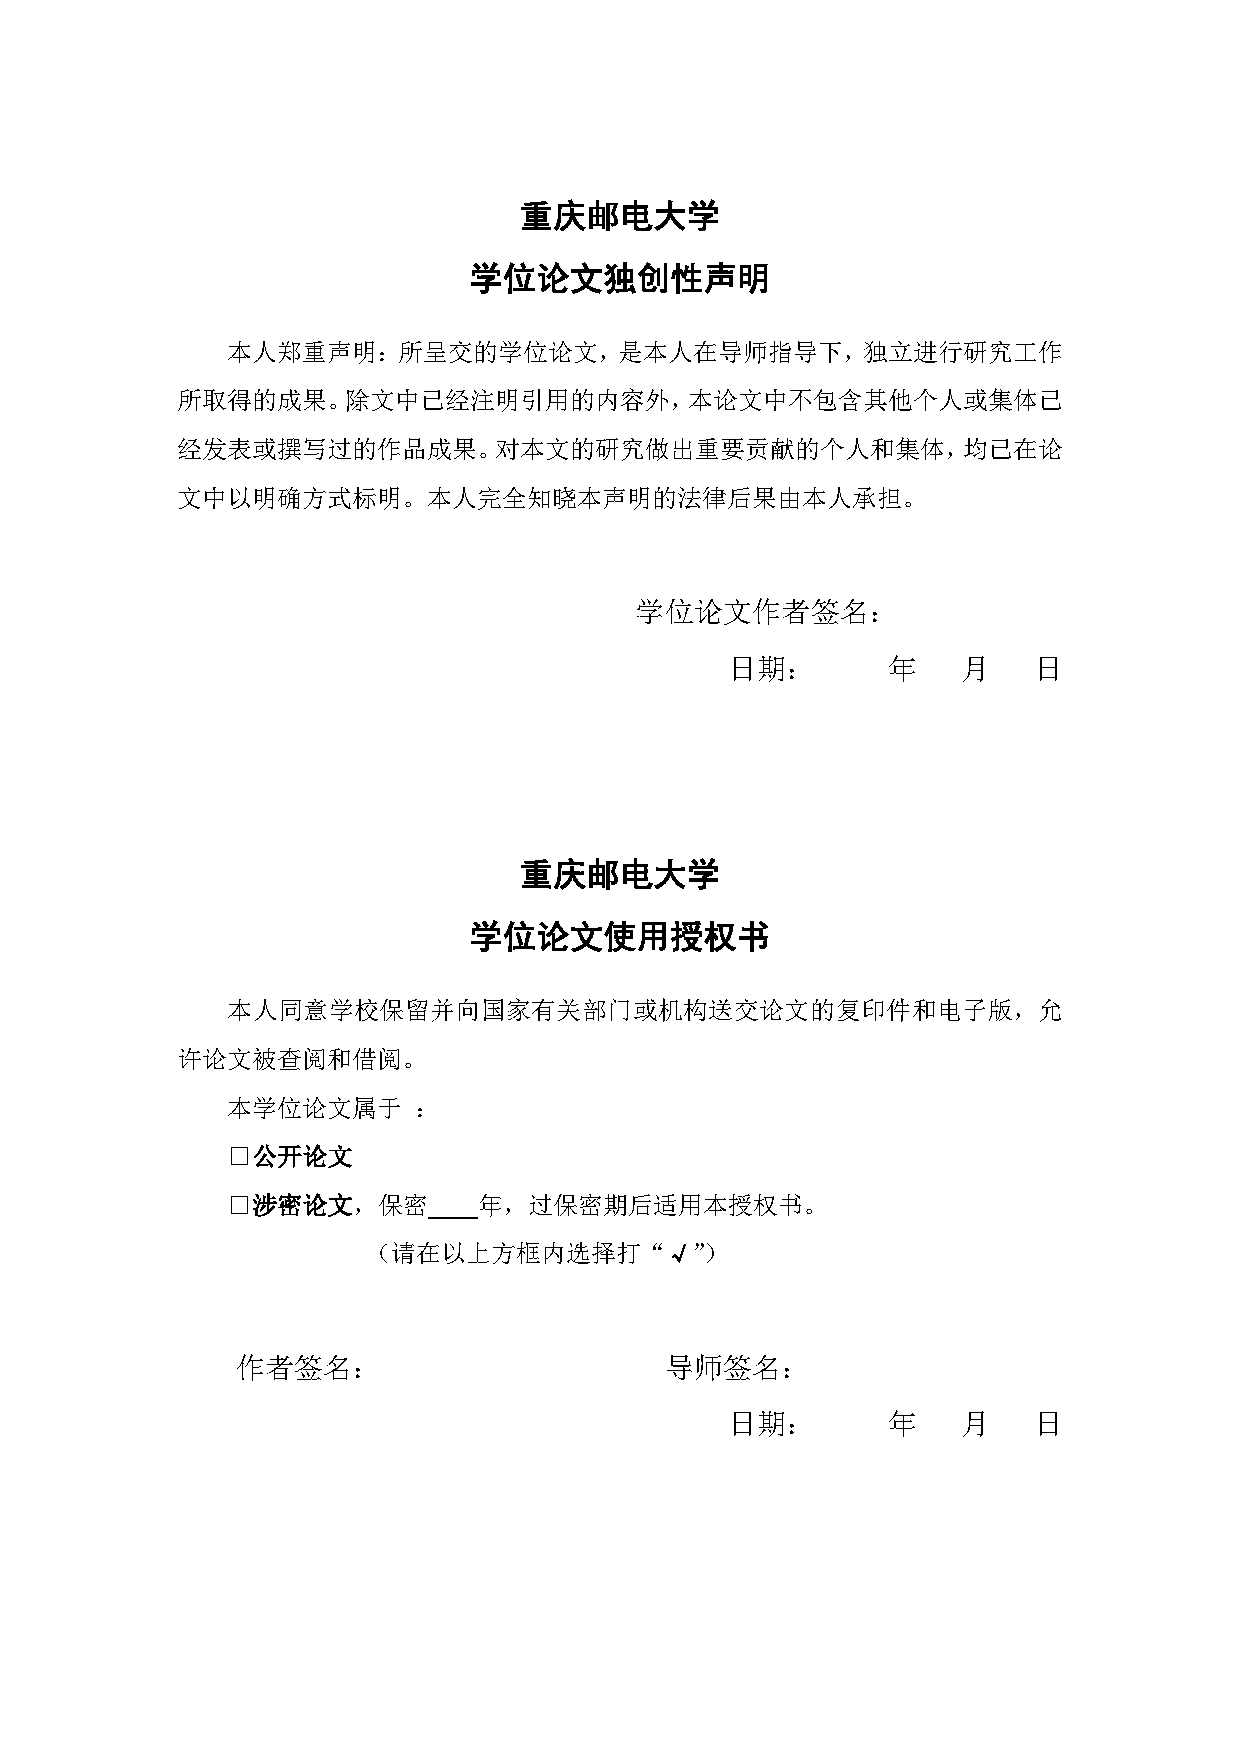
\includepdf{original.pdf}
\clearpage


\clearpage

%前序部分(中英文摘要,目录等,chapter后面不编号)
\frontmatter

%开始以大写罗马字母计页码
\pagenumbering{Roman}

\pagestyle{plain}
%页面格式
%\pagestyle{plain}

% 中文摘要页
%中文摘要,自行编辑内容



\chapter{摘\quad 要}
\xiaosi

学位论文是研究生从事科研工作的成果的主要表现,集中表明了作者在研究工作中获得的新发明、新理论或新见解,是研究生申请硕士或博士学位的重要依据,也是科研领域中的重要文献资料和社会的宝贵财富。

为进一步规范我校研究生学位论文撰写格式,提高研究生学位论文质量,参照国家标准《学位论文编写规则》(GB/T 7713.1-2006),结合我校实际,制定本模板。
\\
  
\noindent\songti\textbf{关键词:}学位论文,撰写规范,论文模板,重庆邮电大学

\clearpage


% 英文摘要页
%英文摘要,自行编辑内容




\chapter{ABSTRACT}
\xiaosi

Dissertation /Thesis is postgraduate’s main academic performance to display her/his works of scientific research, which shows the author’s new invention, new theory or new opinion in her/his research. It is the crucial document for the graduate students to apply for degree, and it is also the important scientific research literature and the valuable wealth of society.

In order to further standardize the format of dissertation/thesis writing and improve graduate dissertation/thesis quality, this temolate is formulated with reference to the national standard "Rules for Dissertation Writing" (GB/T 7713.1-2006) and the reality of CQUPT.
\\

\noindent\textbf{Keywords:} 
\begin{minipage}[t]{0.85\linewidth}
	Dissertation/Thesis, Writing Specification, Thesis Template, Chongqing University of Posts and Telecommunications
\end{minipage}

\clearpage


% 目录
%\begin{spacing}{1.14}
\tableofcontents


\begingroup
\renewcommand*{\addvspace}[1]{}
%图目录
%\newcommand{\loflabel}{图}
%\renewcommand{\numberline}[1]{\loflabel~#1\hspace*{1em}}
\listoffigures

%表目录
%\newcommand{\lotlabel}{表}
%\renewcommand{\numberline}[1]{\lotlabel~#1\hspace*{1em}}
\listoftables
\endgroup

%\end{spacing}





%主要符号表


\chapter{主要符号表}



\begin{table}[h]
	\renewcommand{\arraystretch}{1.5}
	\centering
	\begin{tabular}{p{2cm}p{10cm}p{1.5cm}}
		\toprule[1.5pt]
		\makecell[l]{\songti\xiaosi\bfseries 符号}&\makecell[l]{\songti\xiaosi\bfseries 说明}&\makecell[c]{\songti\xiaosi\bfseries 页码}\\
		\hline
		\makecell[l]{\wuhao c}&\makecell[l]{\wuhao 电磁波的相平面速度}&\makecell[c]{\wuhao 10}\\
		\bottomrule[1.5pt]
	\end{tabular}
     
\end{table}

\clearpage

%缩略词表




\chapter{缩略词表}

\begin{table}[h]
	\renewcommand{\arraystretch}{1.5}
	\centering
	\begin{tabular}{p{2cm}p{8.5cm}p{3cm}}
		\toprule[1.5pt]
		\makecell[l]{\songti\xiaosi\bfseries 英文缩写}&\makecell[l]{\songti\xiaosi\bfseries 英文全称}&\makecell[l]{\songti\xiaosi\bfseries 中文全称}\\
		\hline
		\makecell[l]{\wuhao CQUPT}&\makecell[l]{\wuhao Chongqing University of Posts Telecommunications}&\makecell[l]{\wuhao 重庆邮电大学}\\
		\bottomrule[1.5pt]
	\end{tabular}
	
\end{table}

\clearpage

\clearpage

%% 开始章节写作,chapter后面开始编号,显示特定页眉页脚
\mainmatter
\pagenumbering{arabic}

%正文页眉避免英文全部大写
\renewcommand\thechapter{\arabic{chapter}}
\renewcommand{\chaptermark}[1]{\markboth{第 \thechapter 章 \ #1}{}}




% 第1章



\chapter{绪论}
\thispagestyle{others}
\pagestyle{others}
\xiaosi

\section{研究背景及意义}
学位论文……




\section{国内外研究现状}
学位论文……

\section{论文研究的主要内容}
学位论文……

\section{论文组织结构}
本文……

\clearpage

% 第2章



\chapter{论文结构及文字格式}
\thispagestyle{others}
\pagestyle{others}
\xiaosi

\section{本章引言}

本章引言……

\section{论文结构}

学位论文包括前置部分、主体部分和结尾部分共三大部分,各部分组成及顺序如所示。

学位论文各部分独立为一部分,每部分应从新的一页开始。

论文的正文(中间各章)是论文的核心部分,一般由标题、文字叙述、图、表格和公式等部分构成。由于涉及的学科、选题、研究方法等有很大的差异,可以有不同的写作表达方式,但应遵循本学科通行的学术规范,必须实事求是,客观真切,准确完备,合乎逻辑,层次分明,简练可读。引用他人研究成果时,应注明出处,不得将其与本人的工作混淆。


\section{字数要求}
字数要求


\subsection{硕士论文要求}

各学科和学部自定。

\subsection{博士论文要求}

各学科和学部自定。

\section{字体和段落}
学位论文中的中文统一用宋体,数字和英文统一用Times New Roman字体。从中文摘要开始,所有文字段落和标题行间距均取固定值20磅;所有段落按两端对齐、首行缩进2个全角字符方式书写内容。

中、英文混排时,除小数点以及引用的分图序号、公式序号等外,宜使用全角标点符号(逗号、冒号、括号、引号等);英文段落中,符号使用应遵循英文书写习惯,统一使用半角符号,并规范使用空格。

其他要求:

(1)各级标题不得置于页面的最后一行,即须与下段同页;

(2)两个标题之间无正文时,第二个标题的段前距设置为0磅;

(3)图、表、公式统一采用单倍行距;

(4)只有一、两行文字的,不得单独作为一页内容;除各章最后一页外,中间页面不得出现较大空白;

(5)必要时,可在规定的格式要求基础上适当微调,以利于排版,但显示效果不得与规定的格式要求存在明显差距。

%调整图片与上方文字之间的间距
\vspace{-0.15cm}

\begin{figure}[h]
	\centering 
	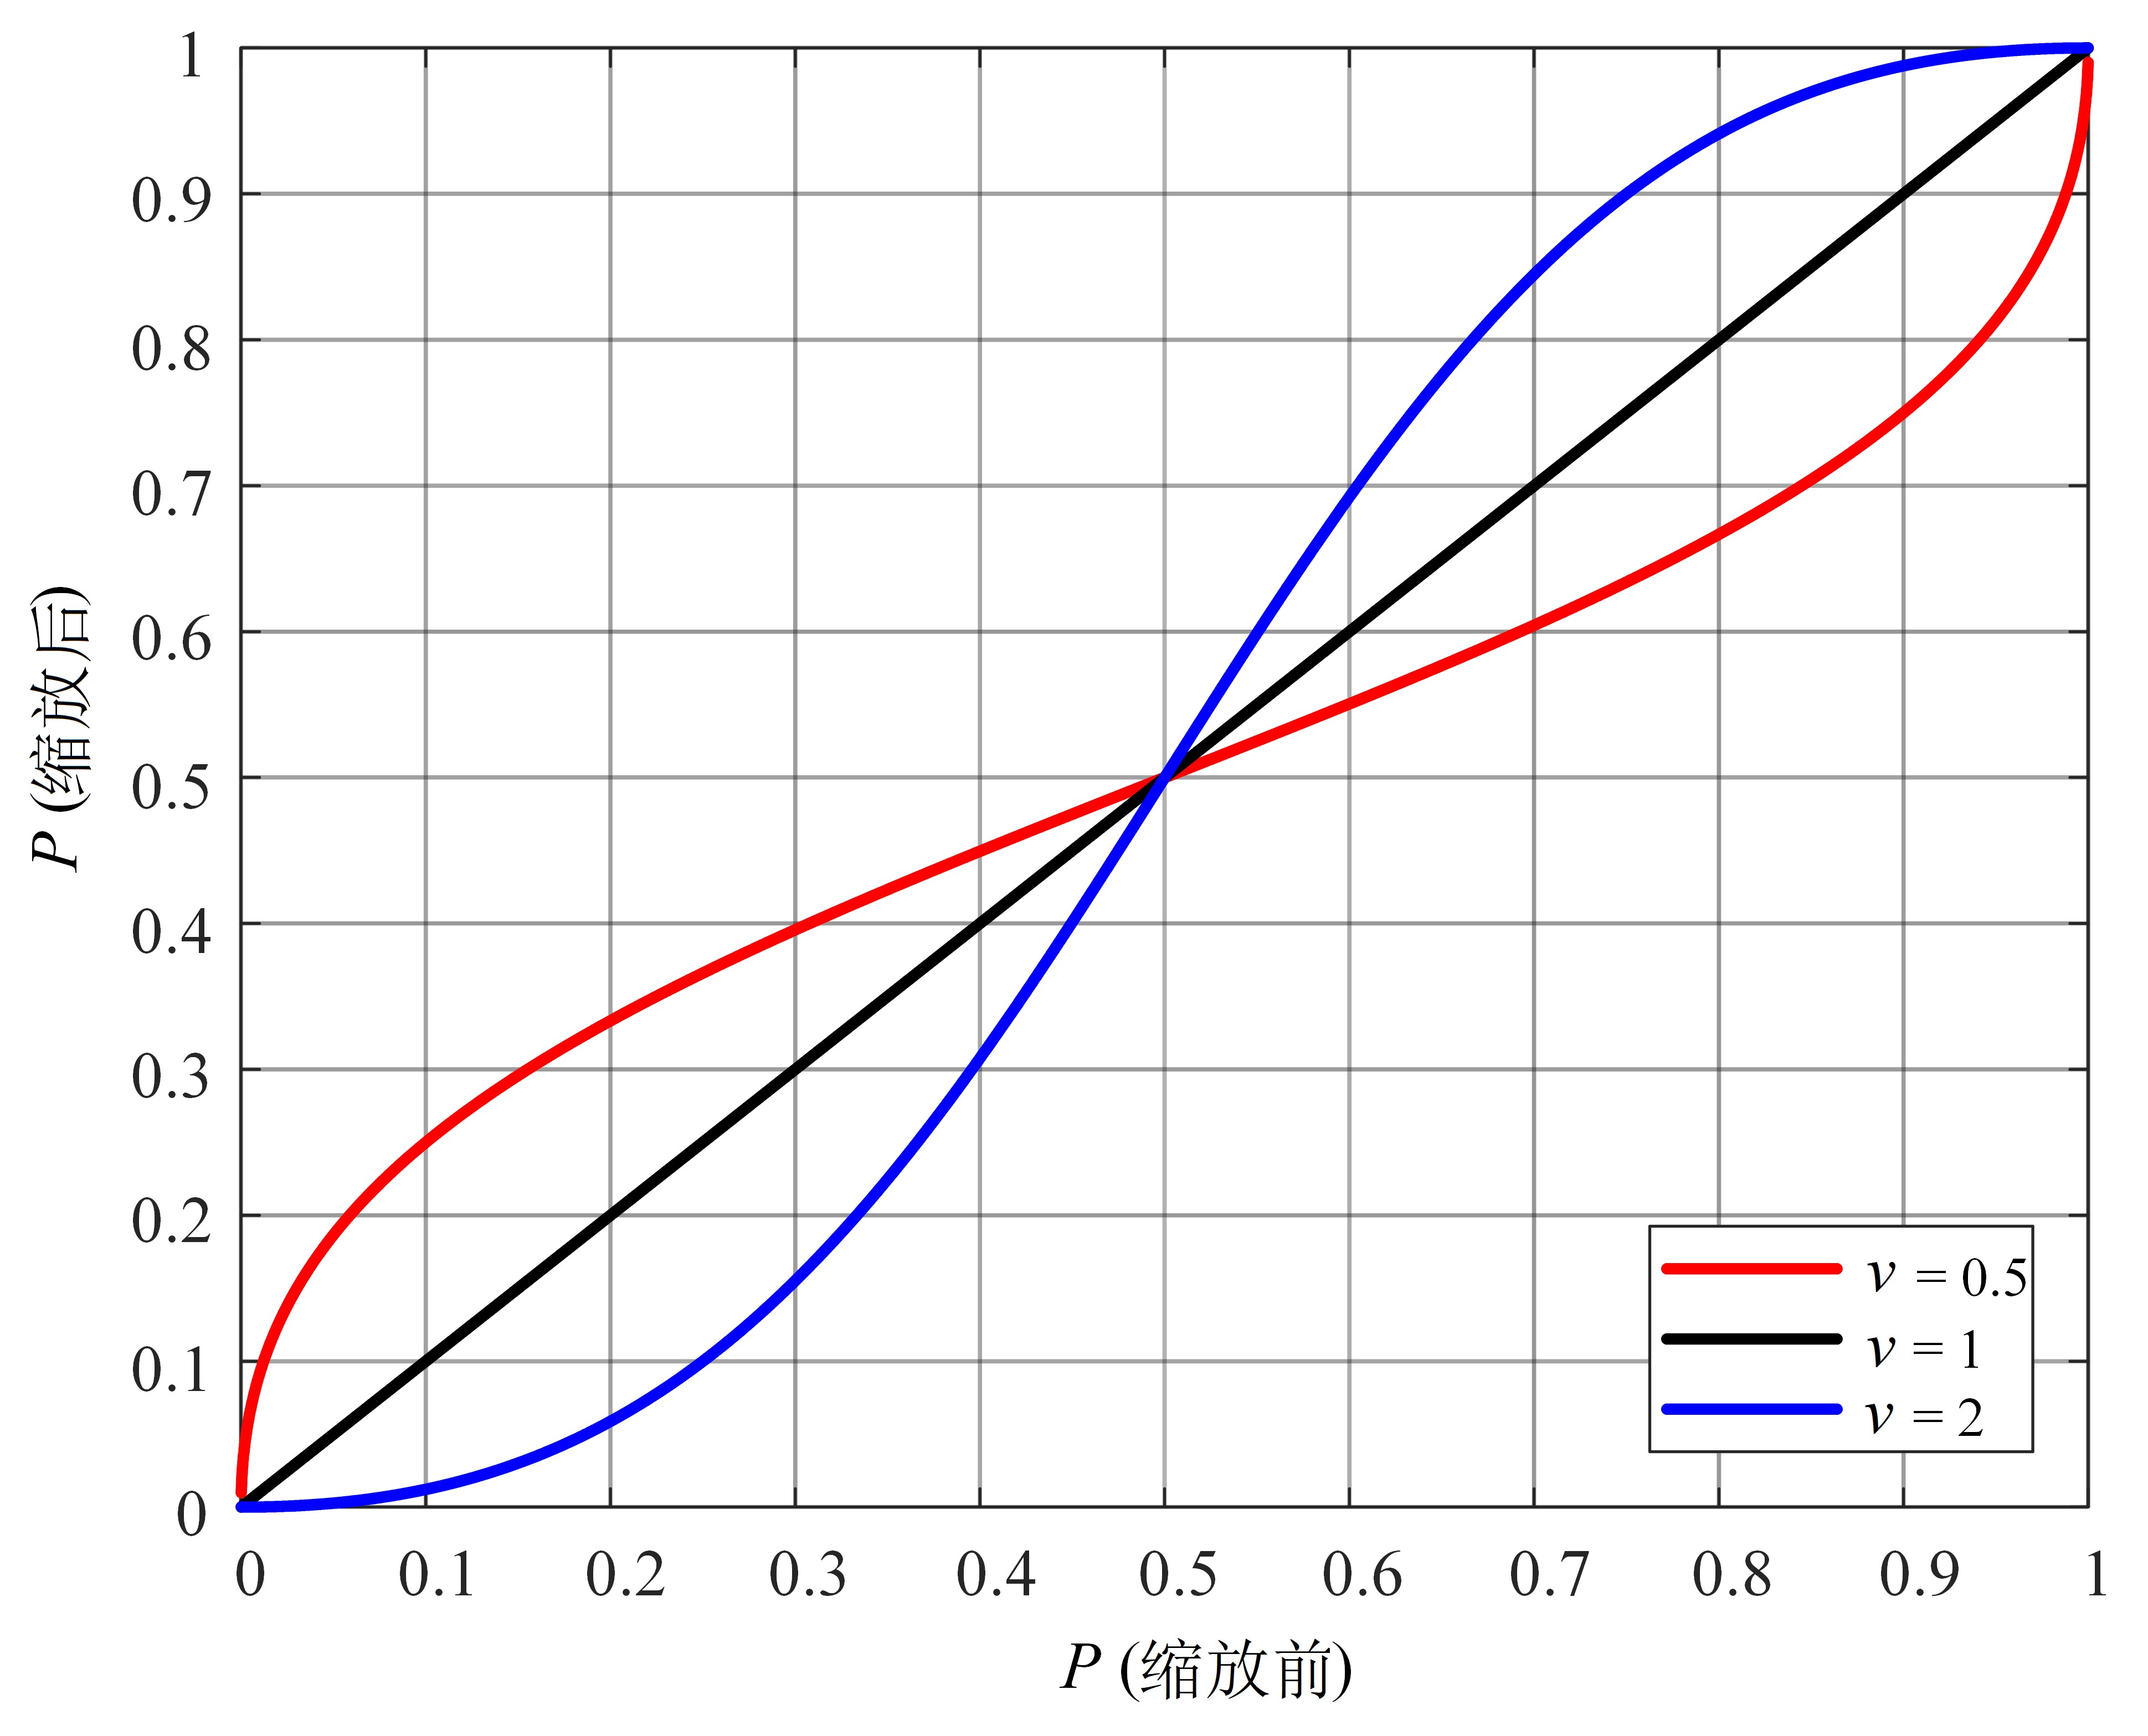
\includegraphics[width=10cm]{chapters/31}
	\bicaption[\xiaosi 不同章节图片排版测试]{\wuhao 图片排版测试}{\wuhao Scaling results with different scaling coefficients ν}
	\label{fig:2.1}
\end{figure}

%调整图片与下方文字之间的间距
\vspace{-0.5cm}

\section{章节标题}
目录中章节标题只显示到3级标题,正文中最多显示到4级标题。

\subsection{三级标题}

\vspace{0.5cm}

\subsubsection{四级标题}

\vspace{0.3cm}



\section{本章小结}
本章介绍了……






% 第3章


\chapter{图表、公式格式和印制要求Abc}
\thispagestyle{others}
\pagestyle{others}
\xiaosi

\section{本章引言}
本章引言……

\section{引用参考文献}
参考文献引用示例:单篇引用\textsuperscript{\cite{ref1}},多篇同处引用\textsuperscript{\cite{ref1,ref2,ref3,ref13}}


\section{图和表格式}

图、表在版面中居中放置,图编号和图题居中列在图下。编号采用阿拉伯数字分章连续编号,例如“图 \ref{fig:3.1}”,“表 \ref{tab:3.1}”以及“式 \ref{eq:3.1}”。

\subsection{图}
下面给出图片示例:

%调整图片与上方文字之间的间距
\vspace{-0.1cm}

\begin{figure}[h]
		\centering 
		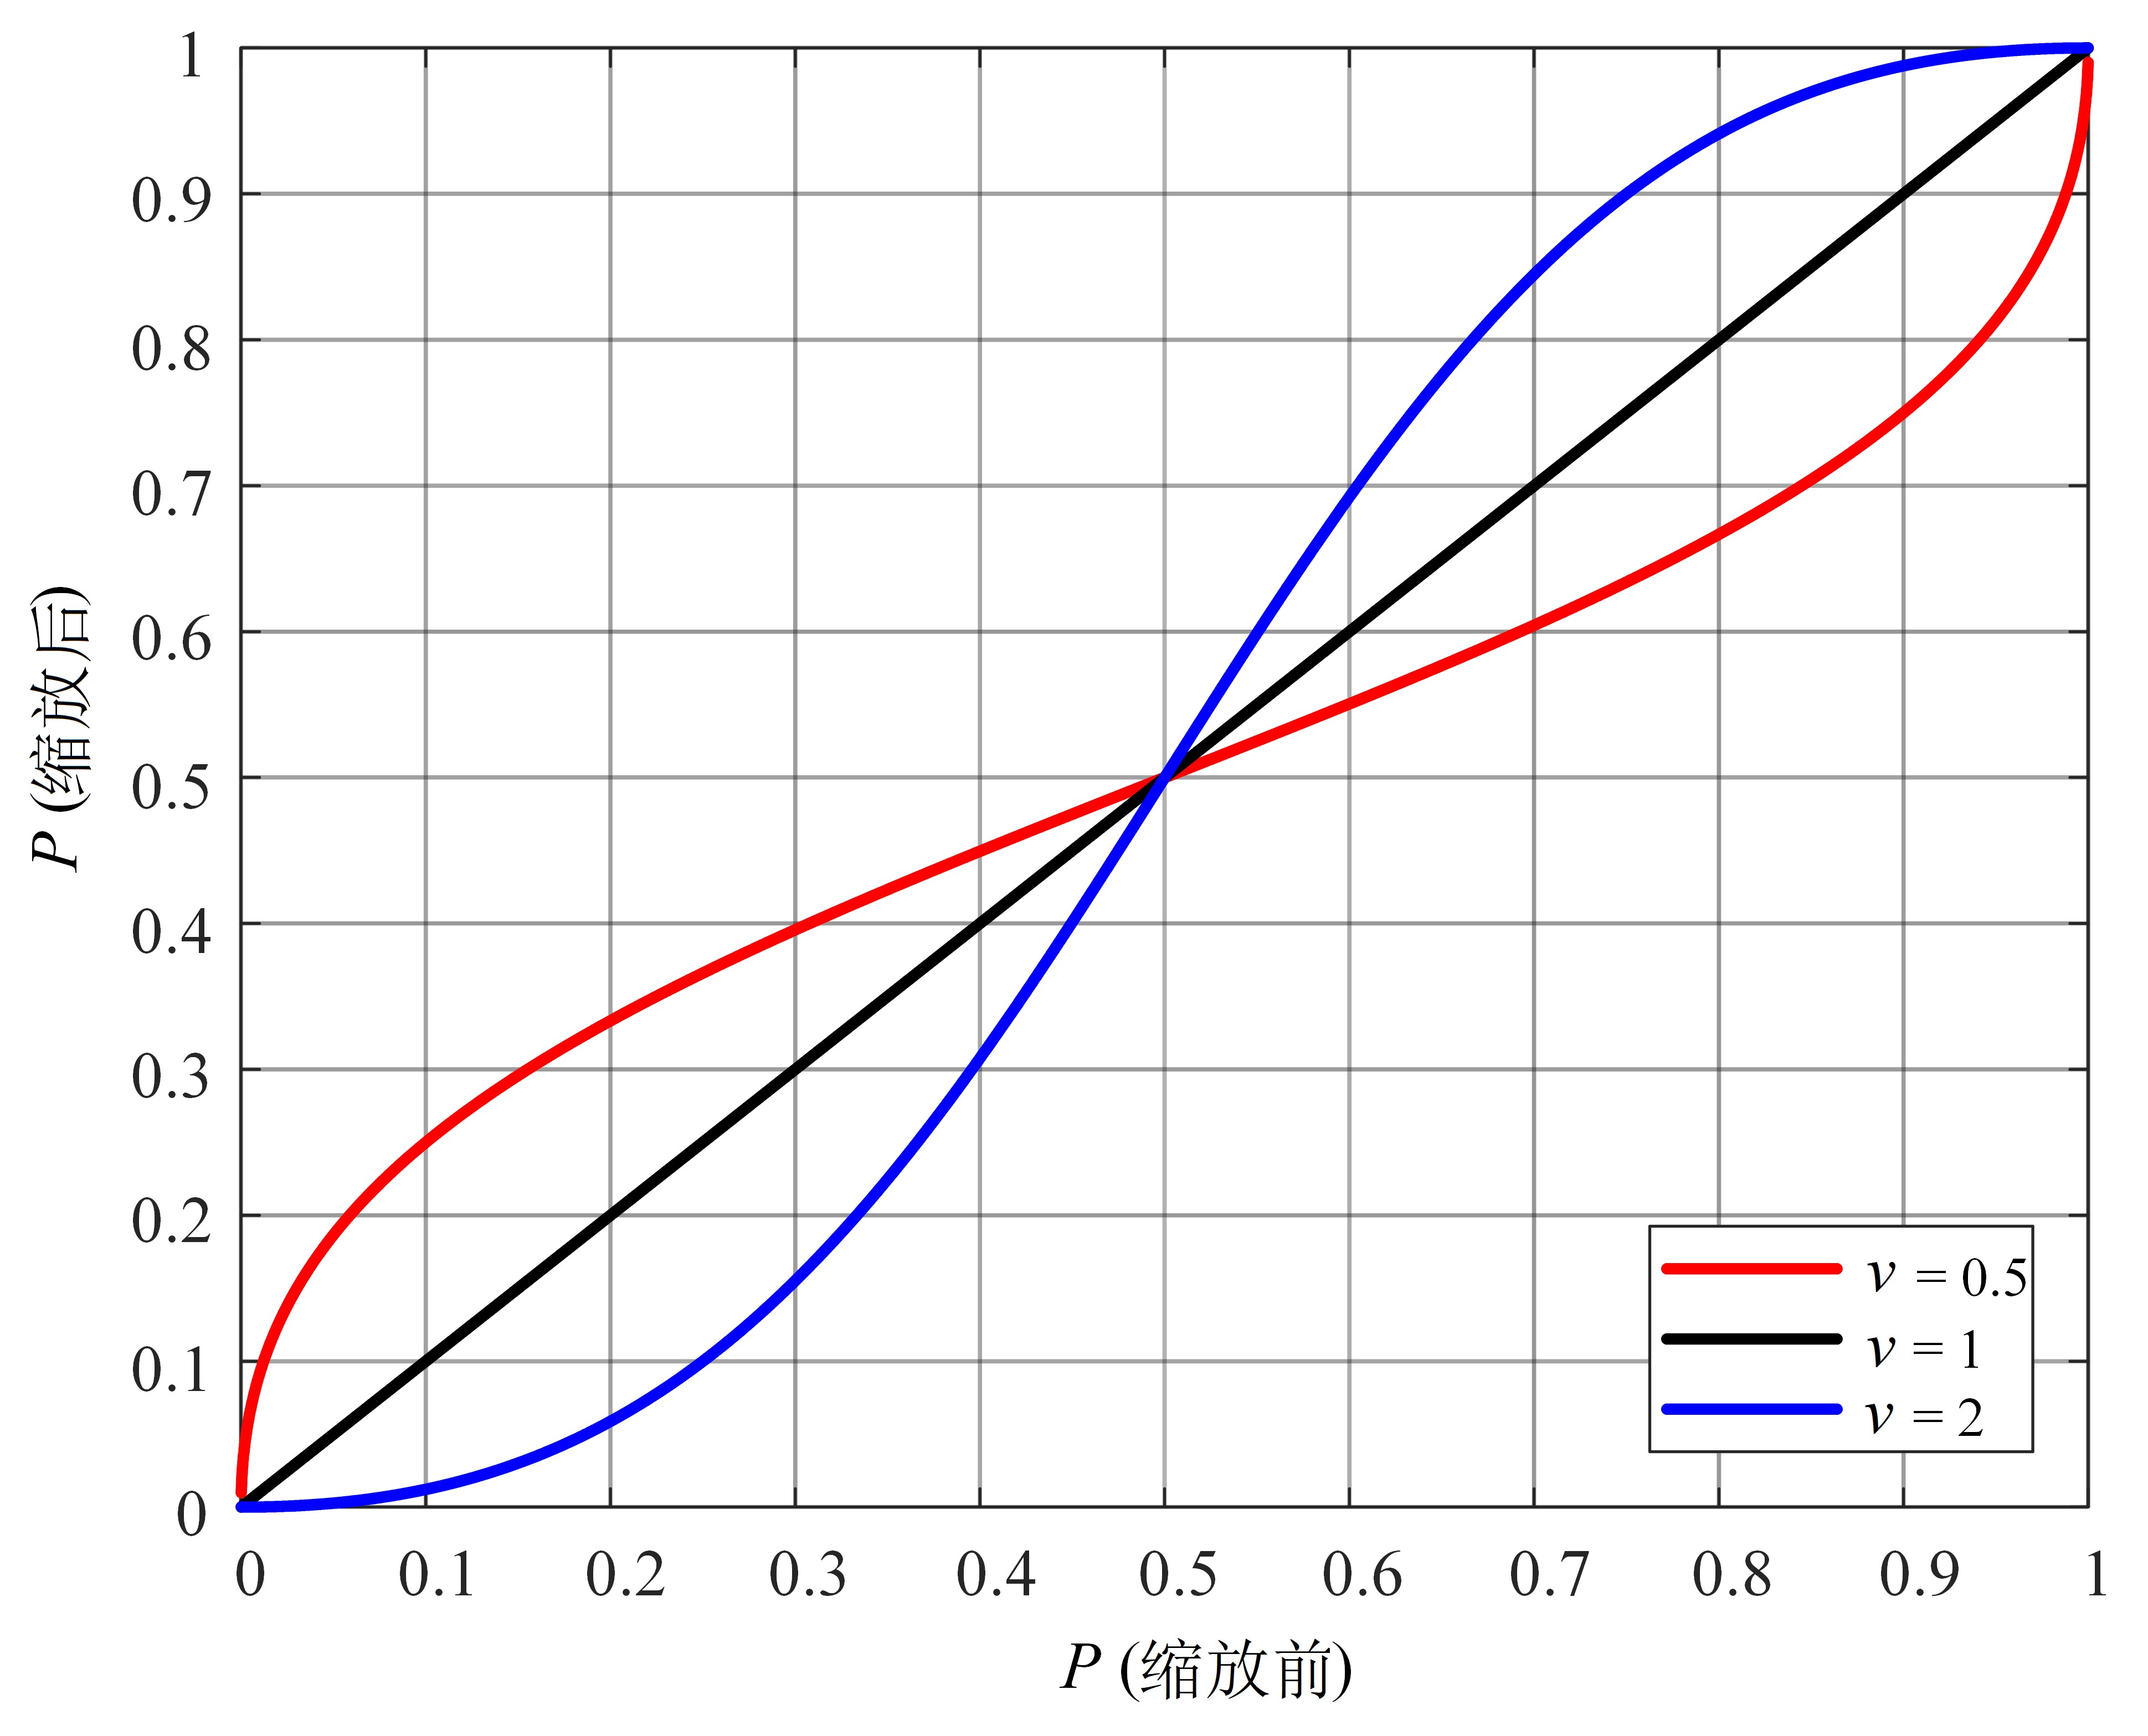
\includegraphics[width=10cm]{chapters/31}
	    \bicaption[\xiaosi 不同缩放系数v的缩放效果]{\wuhao 不同缩放系数v的缩放结果}{\wuhao Scaling results with different scaling coefficients ν}
	   	 \label{fig:3.1}
\end{figure}

%调整图片与下方文字之间的间距
\vspace{-0.35cm}

图片标题与图片之间的间距使用默认设置即可,与上下文的间距由于LATEX动态排版特性,和该页的整体布局有关,需要大家手动调整。

。

。





下图是多子图示例,对于标题没有超过一行的图题,可以参照下面代码进行设置:

\vspace{0.5cm} %调整图片与上文的间距

\begin{figure}[!h]
	\centering
	\subfigure[]{
		\label{fig:666}
		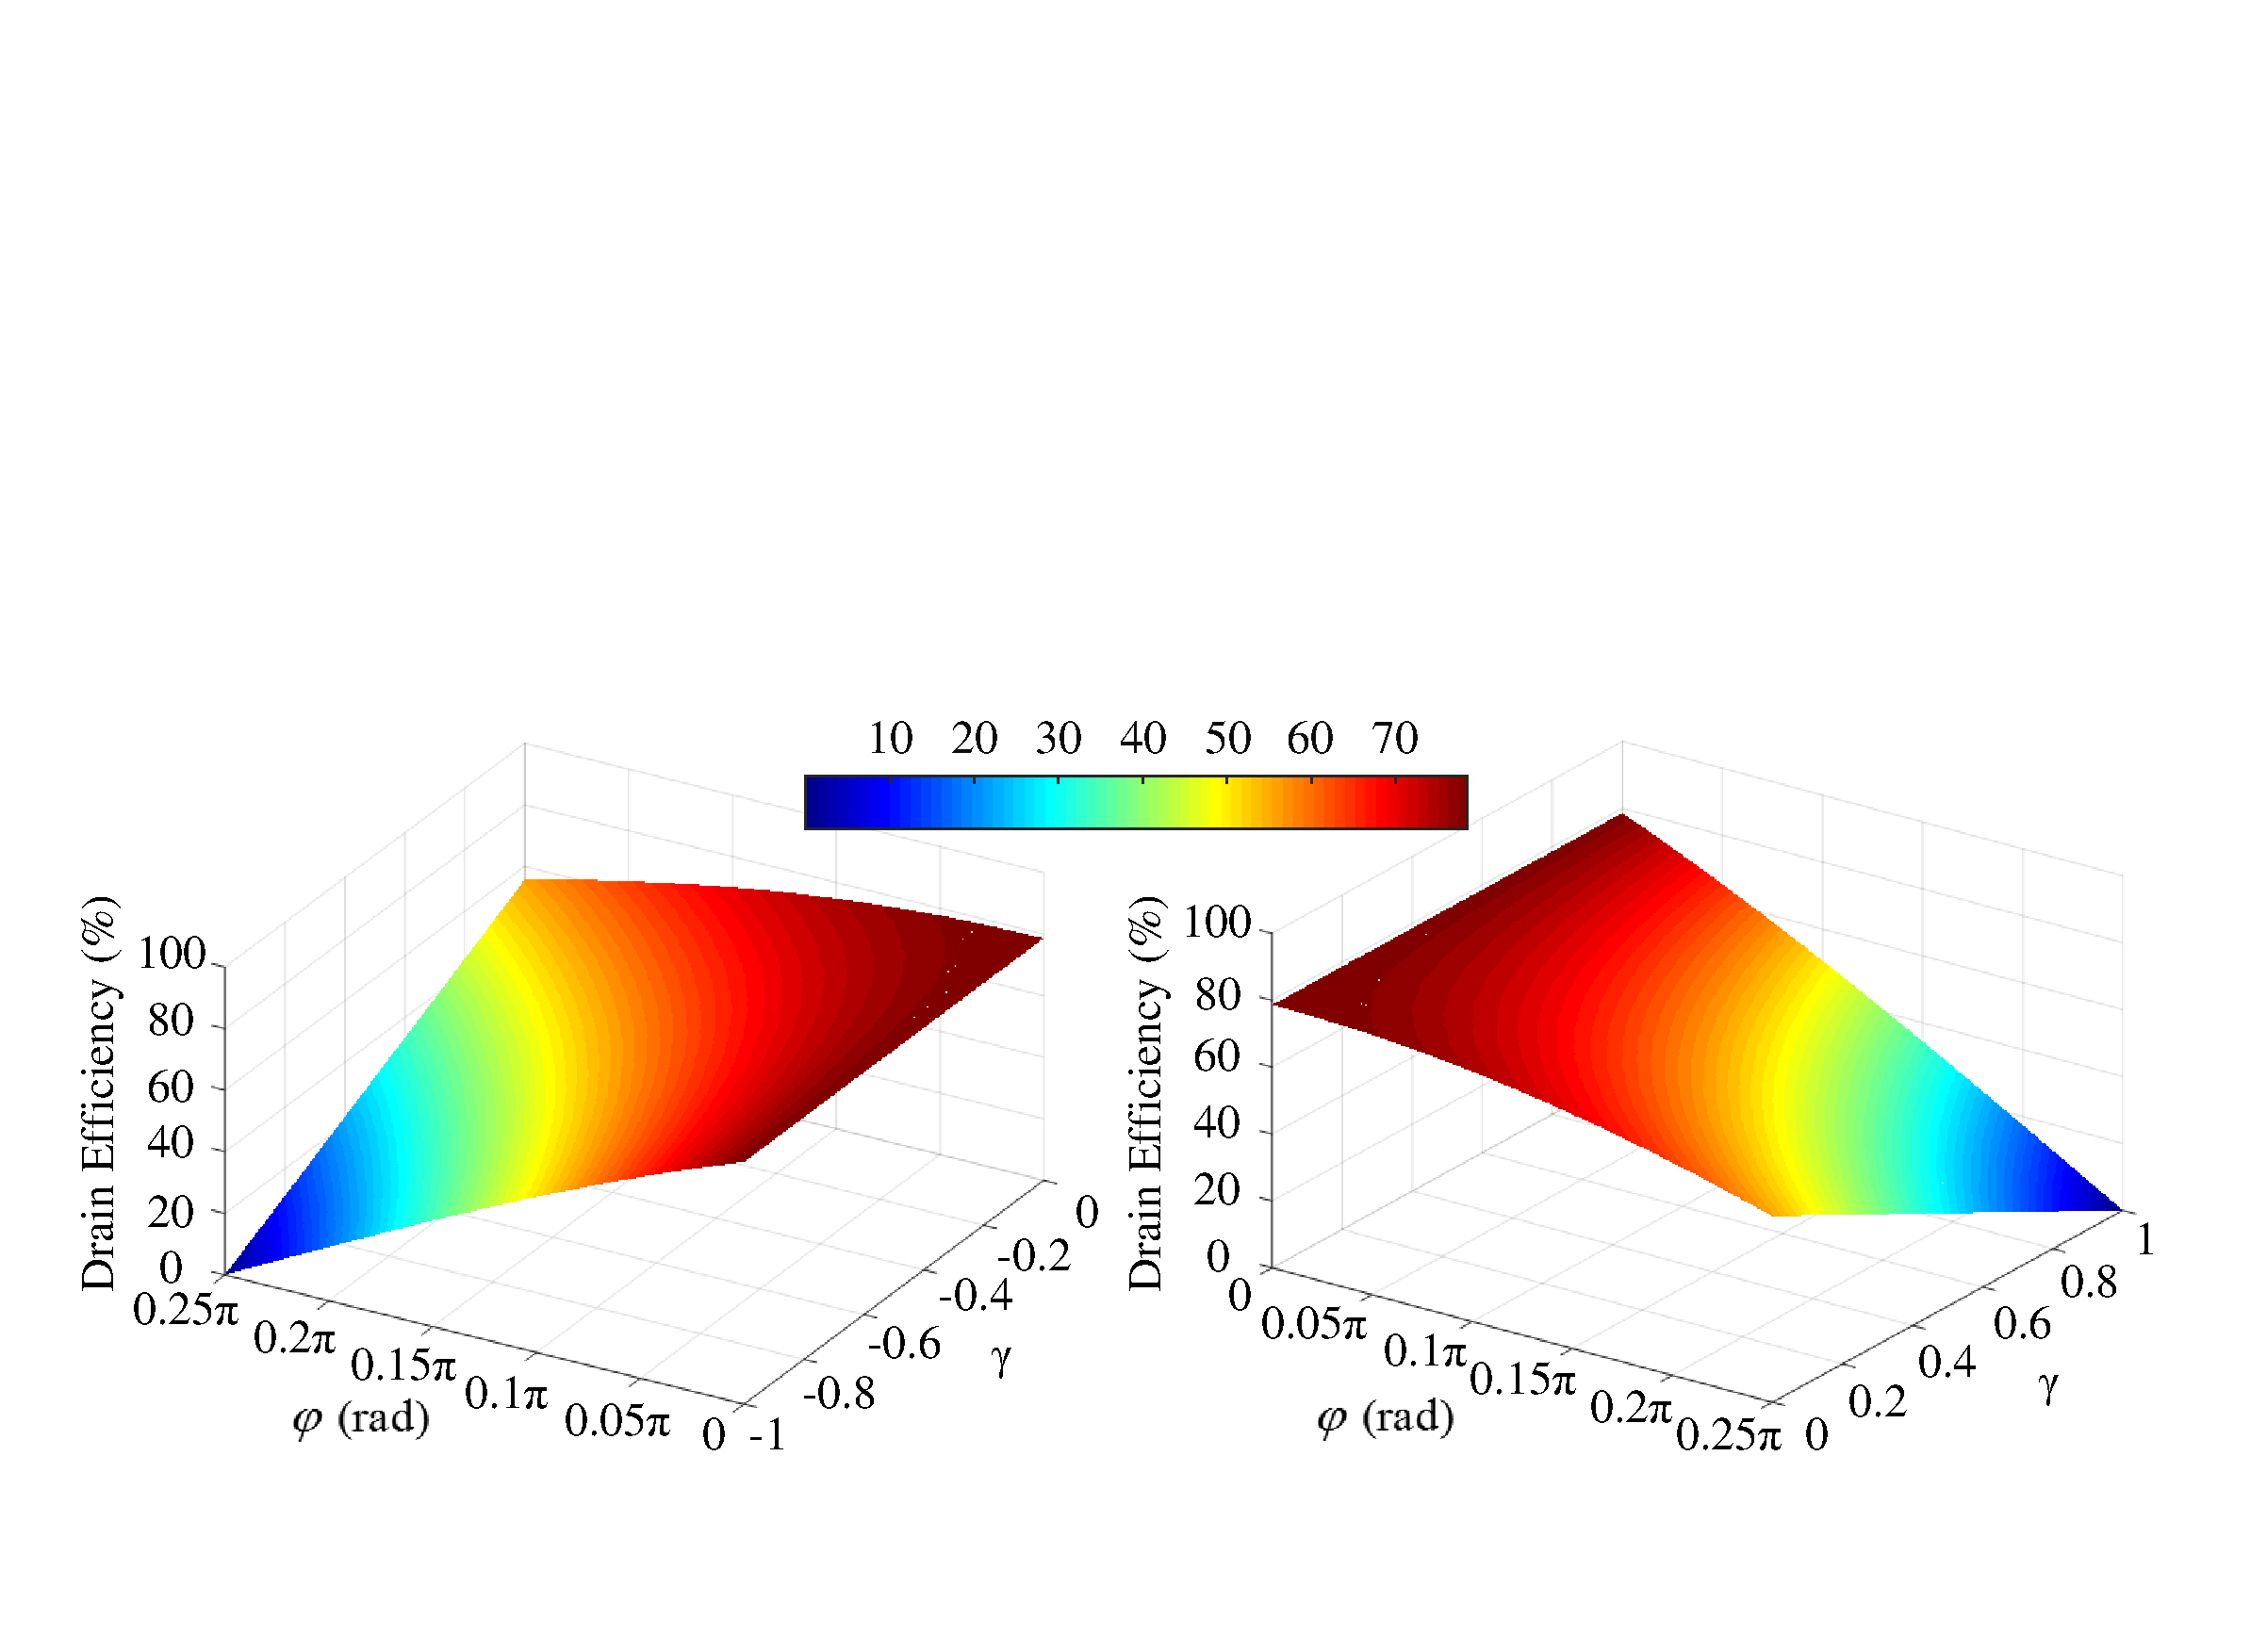
\includegraphics[width=12cm]{chapters/DE_J.pdf}}
	\subfigure[]{
		\label{fig:888}
		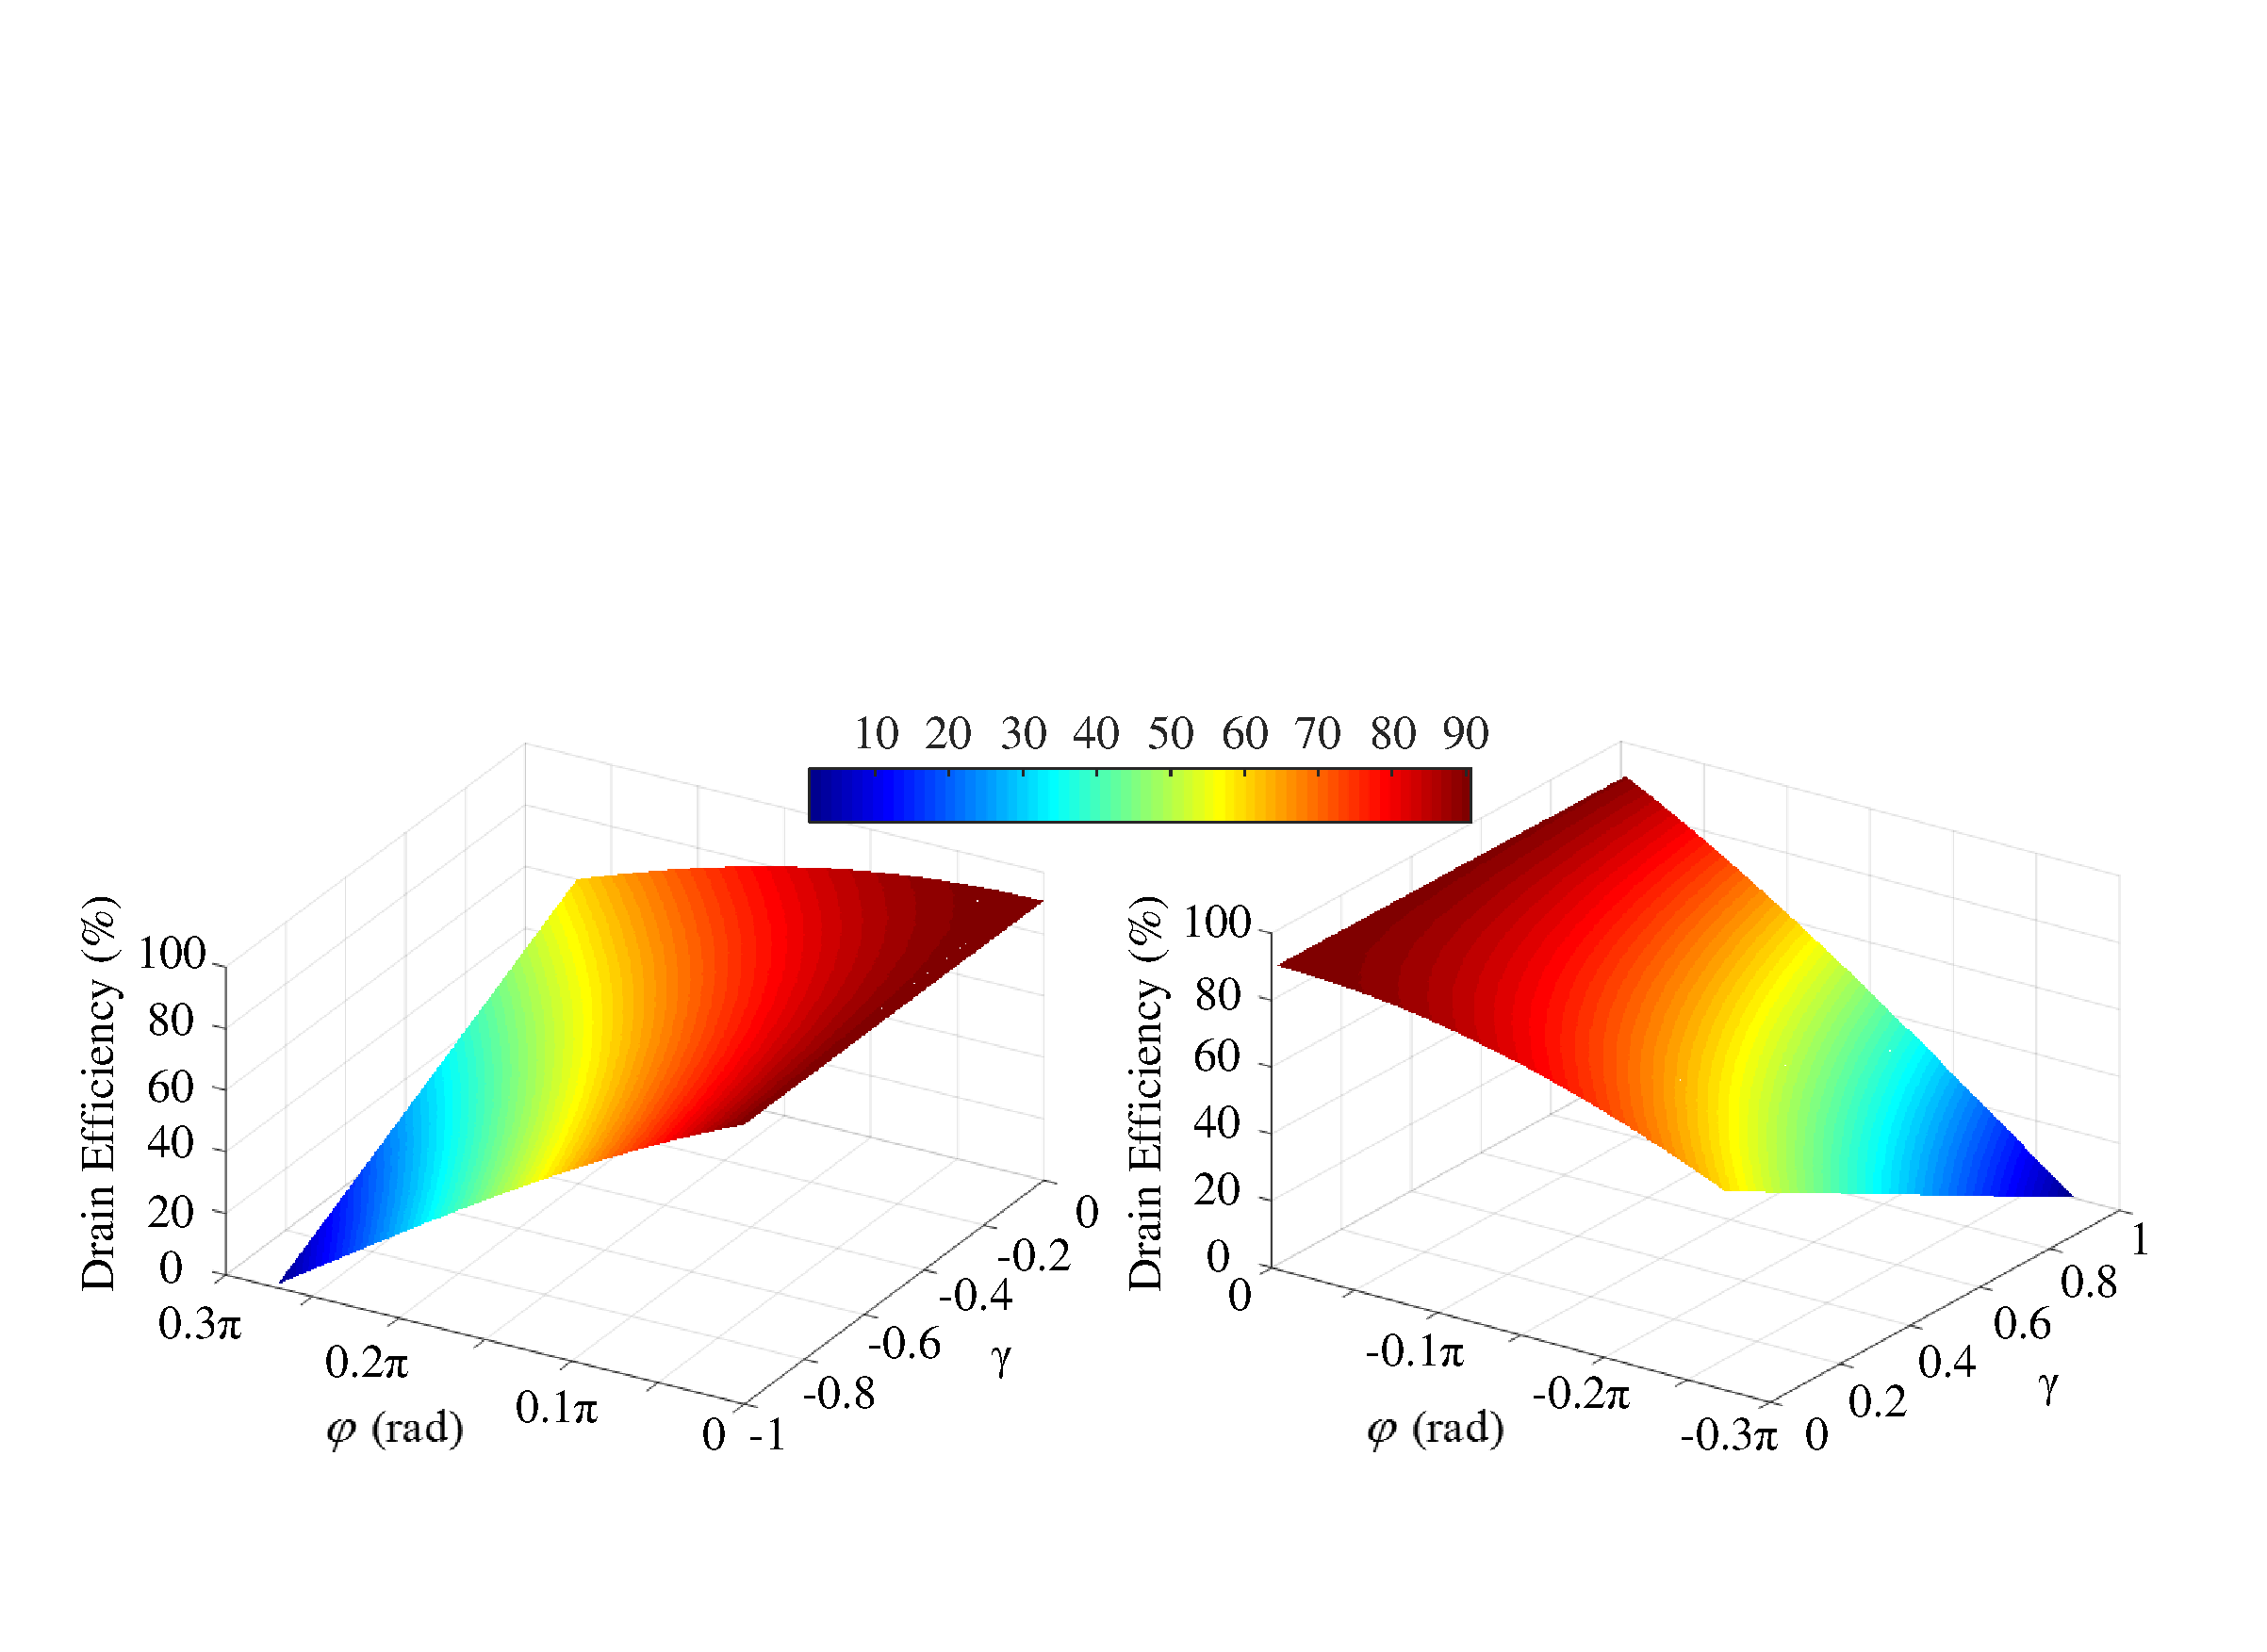
\includegraphics[width=12cm]{chapters/DE_CF.pdf}}
		\bicaption[\xiaosi 理论效率与$\gamma$和$\varphi$的关系]{\wuhao 理论效率与$\gamma$和$\varphi$的关系。 (a) $\alpha=1$; (b) $\alpha=2/\sqrt{3}$}{\wuhao Theoretical DE versus $\gamma$ and $\varphi$. (a) $\alpha=1$; (b) $\alpha=2/\sqrt{3}$}
\end{figure}

\vspace{-0.2cm} %调整图片与下文的间距

图片要求参照写作指南。图片要求参照写作指南。图片要求参照写作指南。图片要求参照写作指南。图片要求参照写作指南。图片要求参照写作指南。图片要求参照写作指南。图片要求参照写作指南。图片要求参照写作指南。图片要求参照写作指南。图片要求参照写作指南。图片要求参照写作指南。图片要求参照写作指南。图片要求参照写作指南。

图片要求参照写作指南。图片要求参照写作指南。图片要求参照写作指南。图片要求参照写作指南。图片要求参照写作指南。图片要求参照写作指南。图片要求参照写作指南。图片要求参照写作指南。图片要求参照写作指南。图片要求参照写作指南。图片要求参照写作指南。图片要求参照写作指南。图片要求参照写作指南。图片要求参照写作指南。图片要求参照写作指南。图片要求参照写作指南。图片要求参照写作指南。图片要求参照写作指南。图片要求参照写作指南。图片要求参照写作指南。图片要求参照写作指南。


对于图题超过了一行的图片,请参照下面代码进行设置,使得图题能与WORD一样居中左对齐,注意其中bicaption[]()(这个里面的字号使用wuhaob):

\vspace{0.3cm}

\begin{figure}[!h]
	\centering
	\subfigure[]{
		\label{fig:DE_J}
		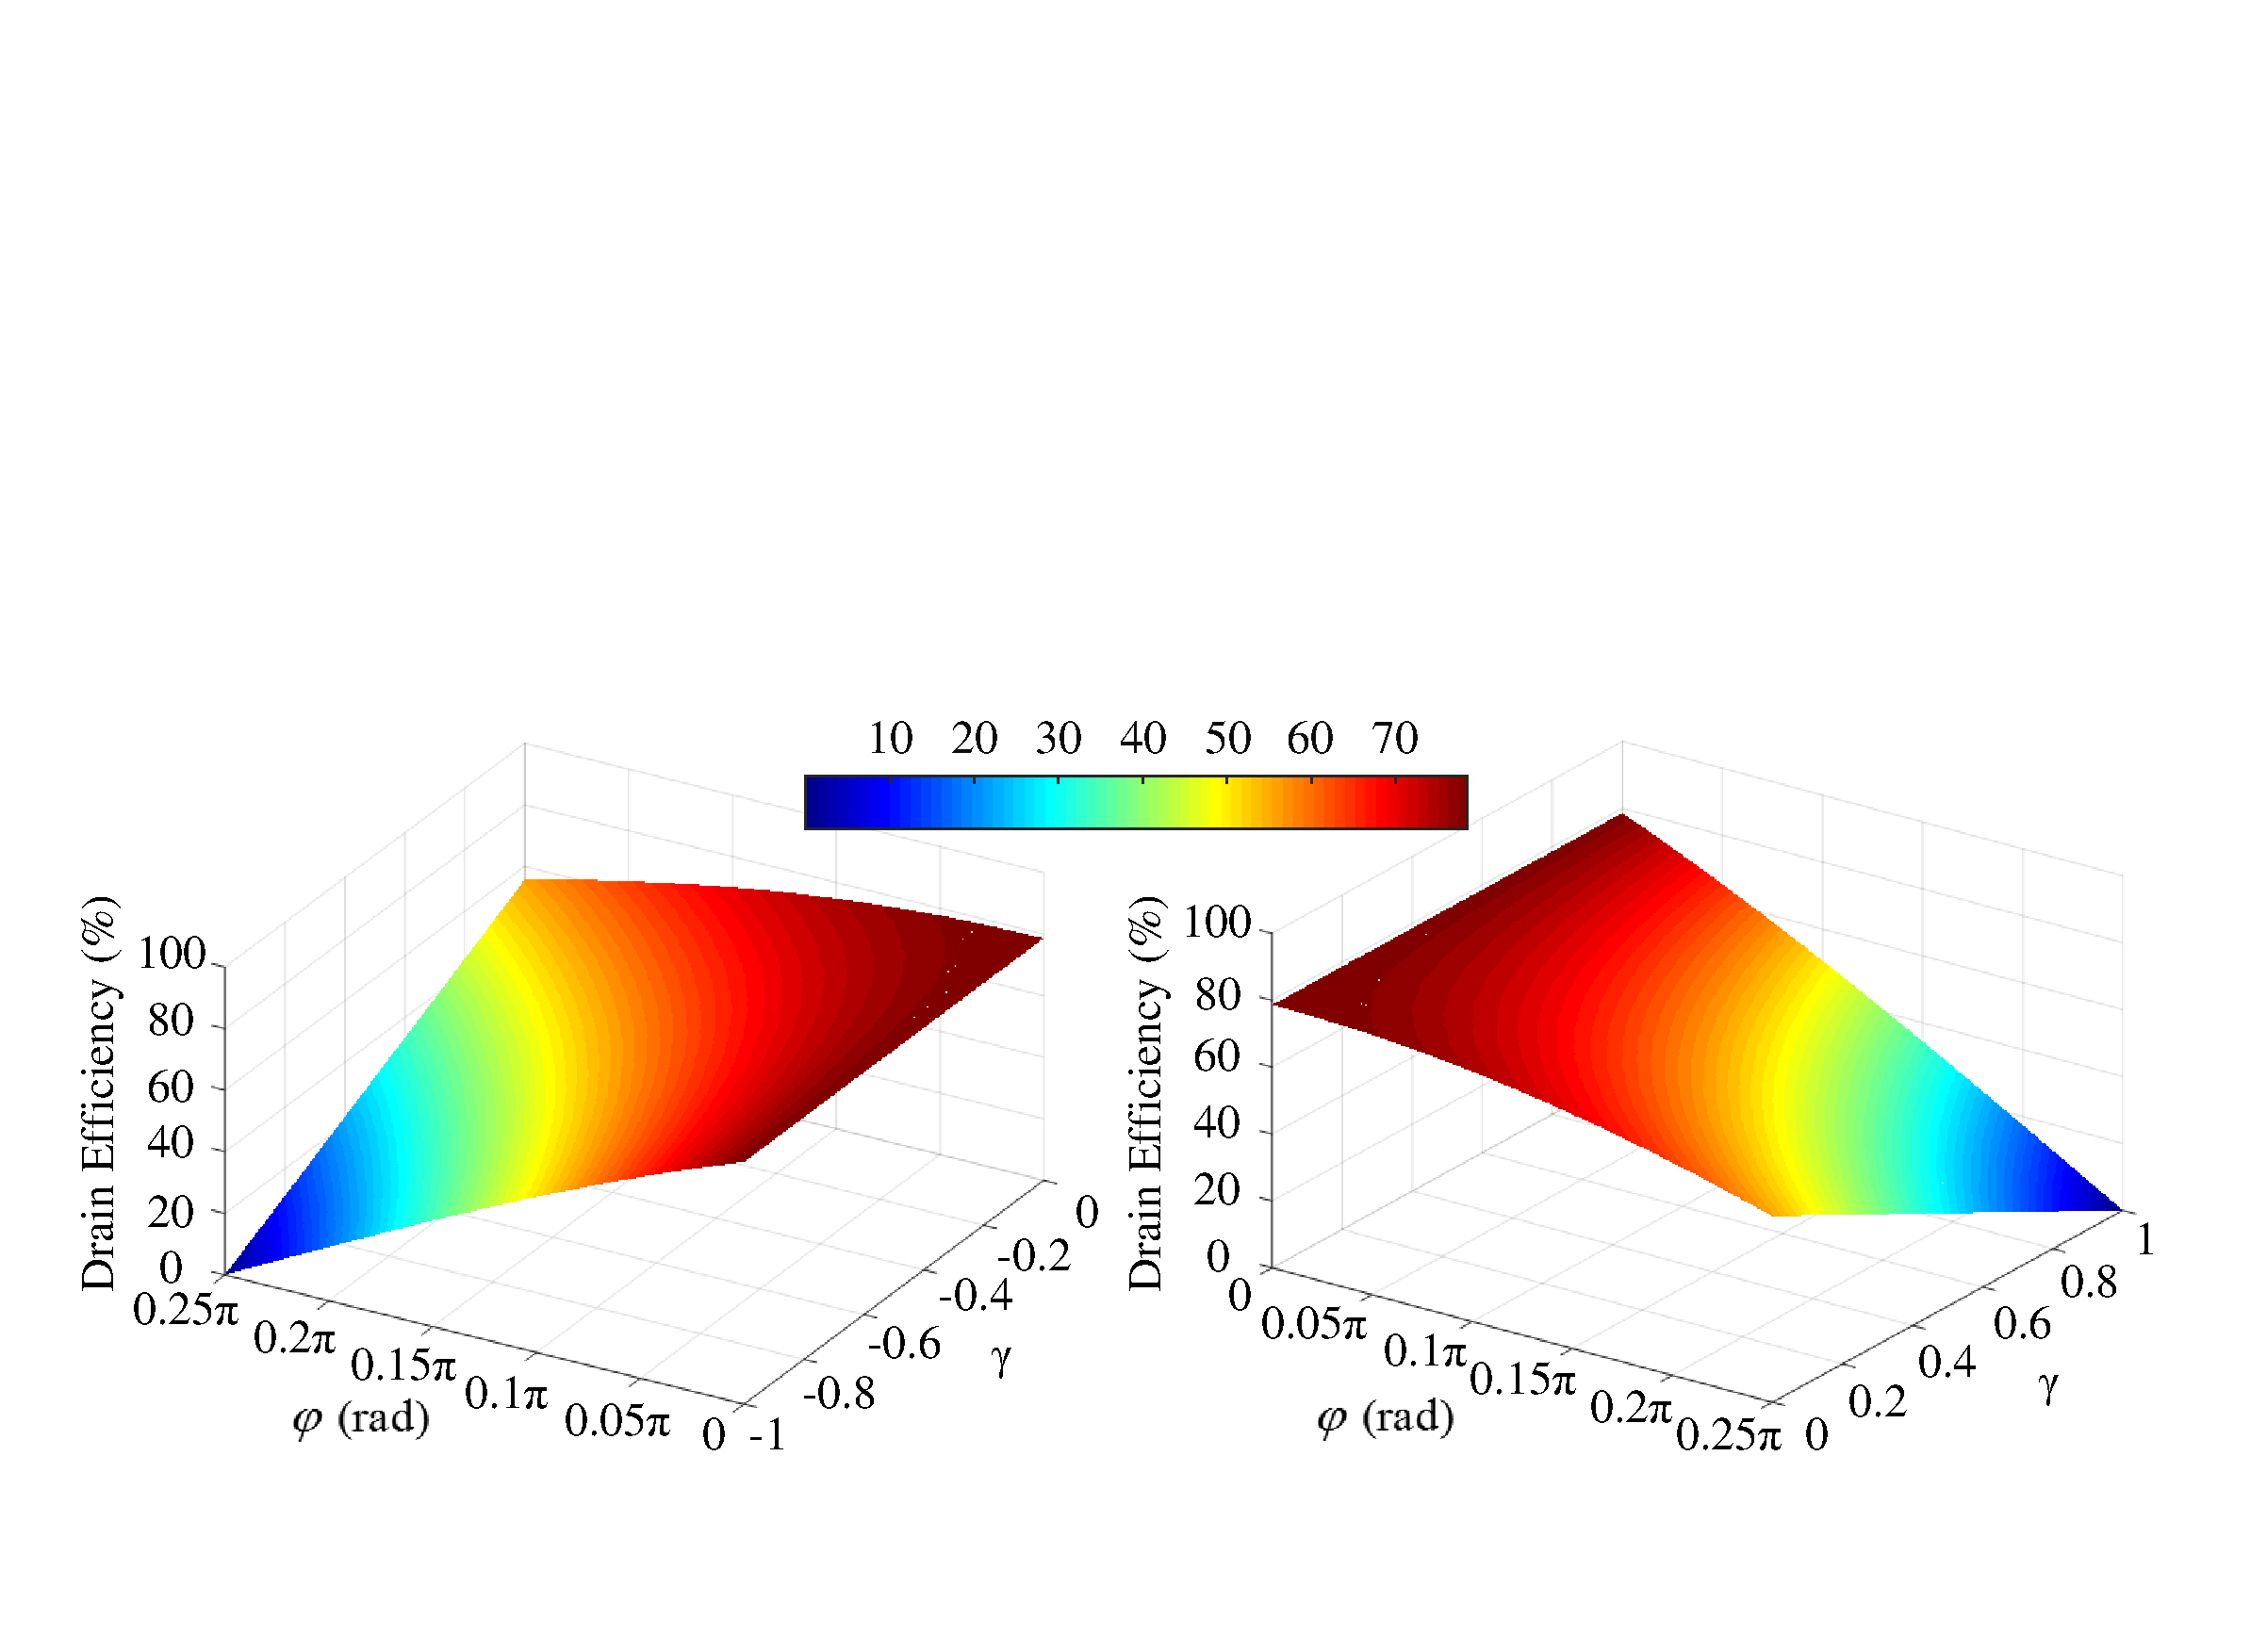
\includegraphics[width=12cm]{chapters/DE_J.pdf}}
	\subfigure[]{
		\label{fig:DE_CF}
		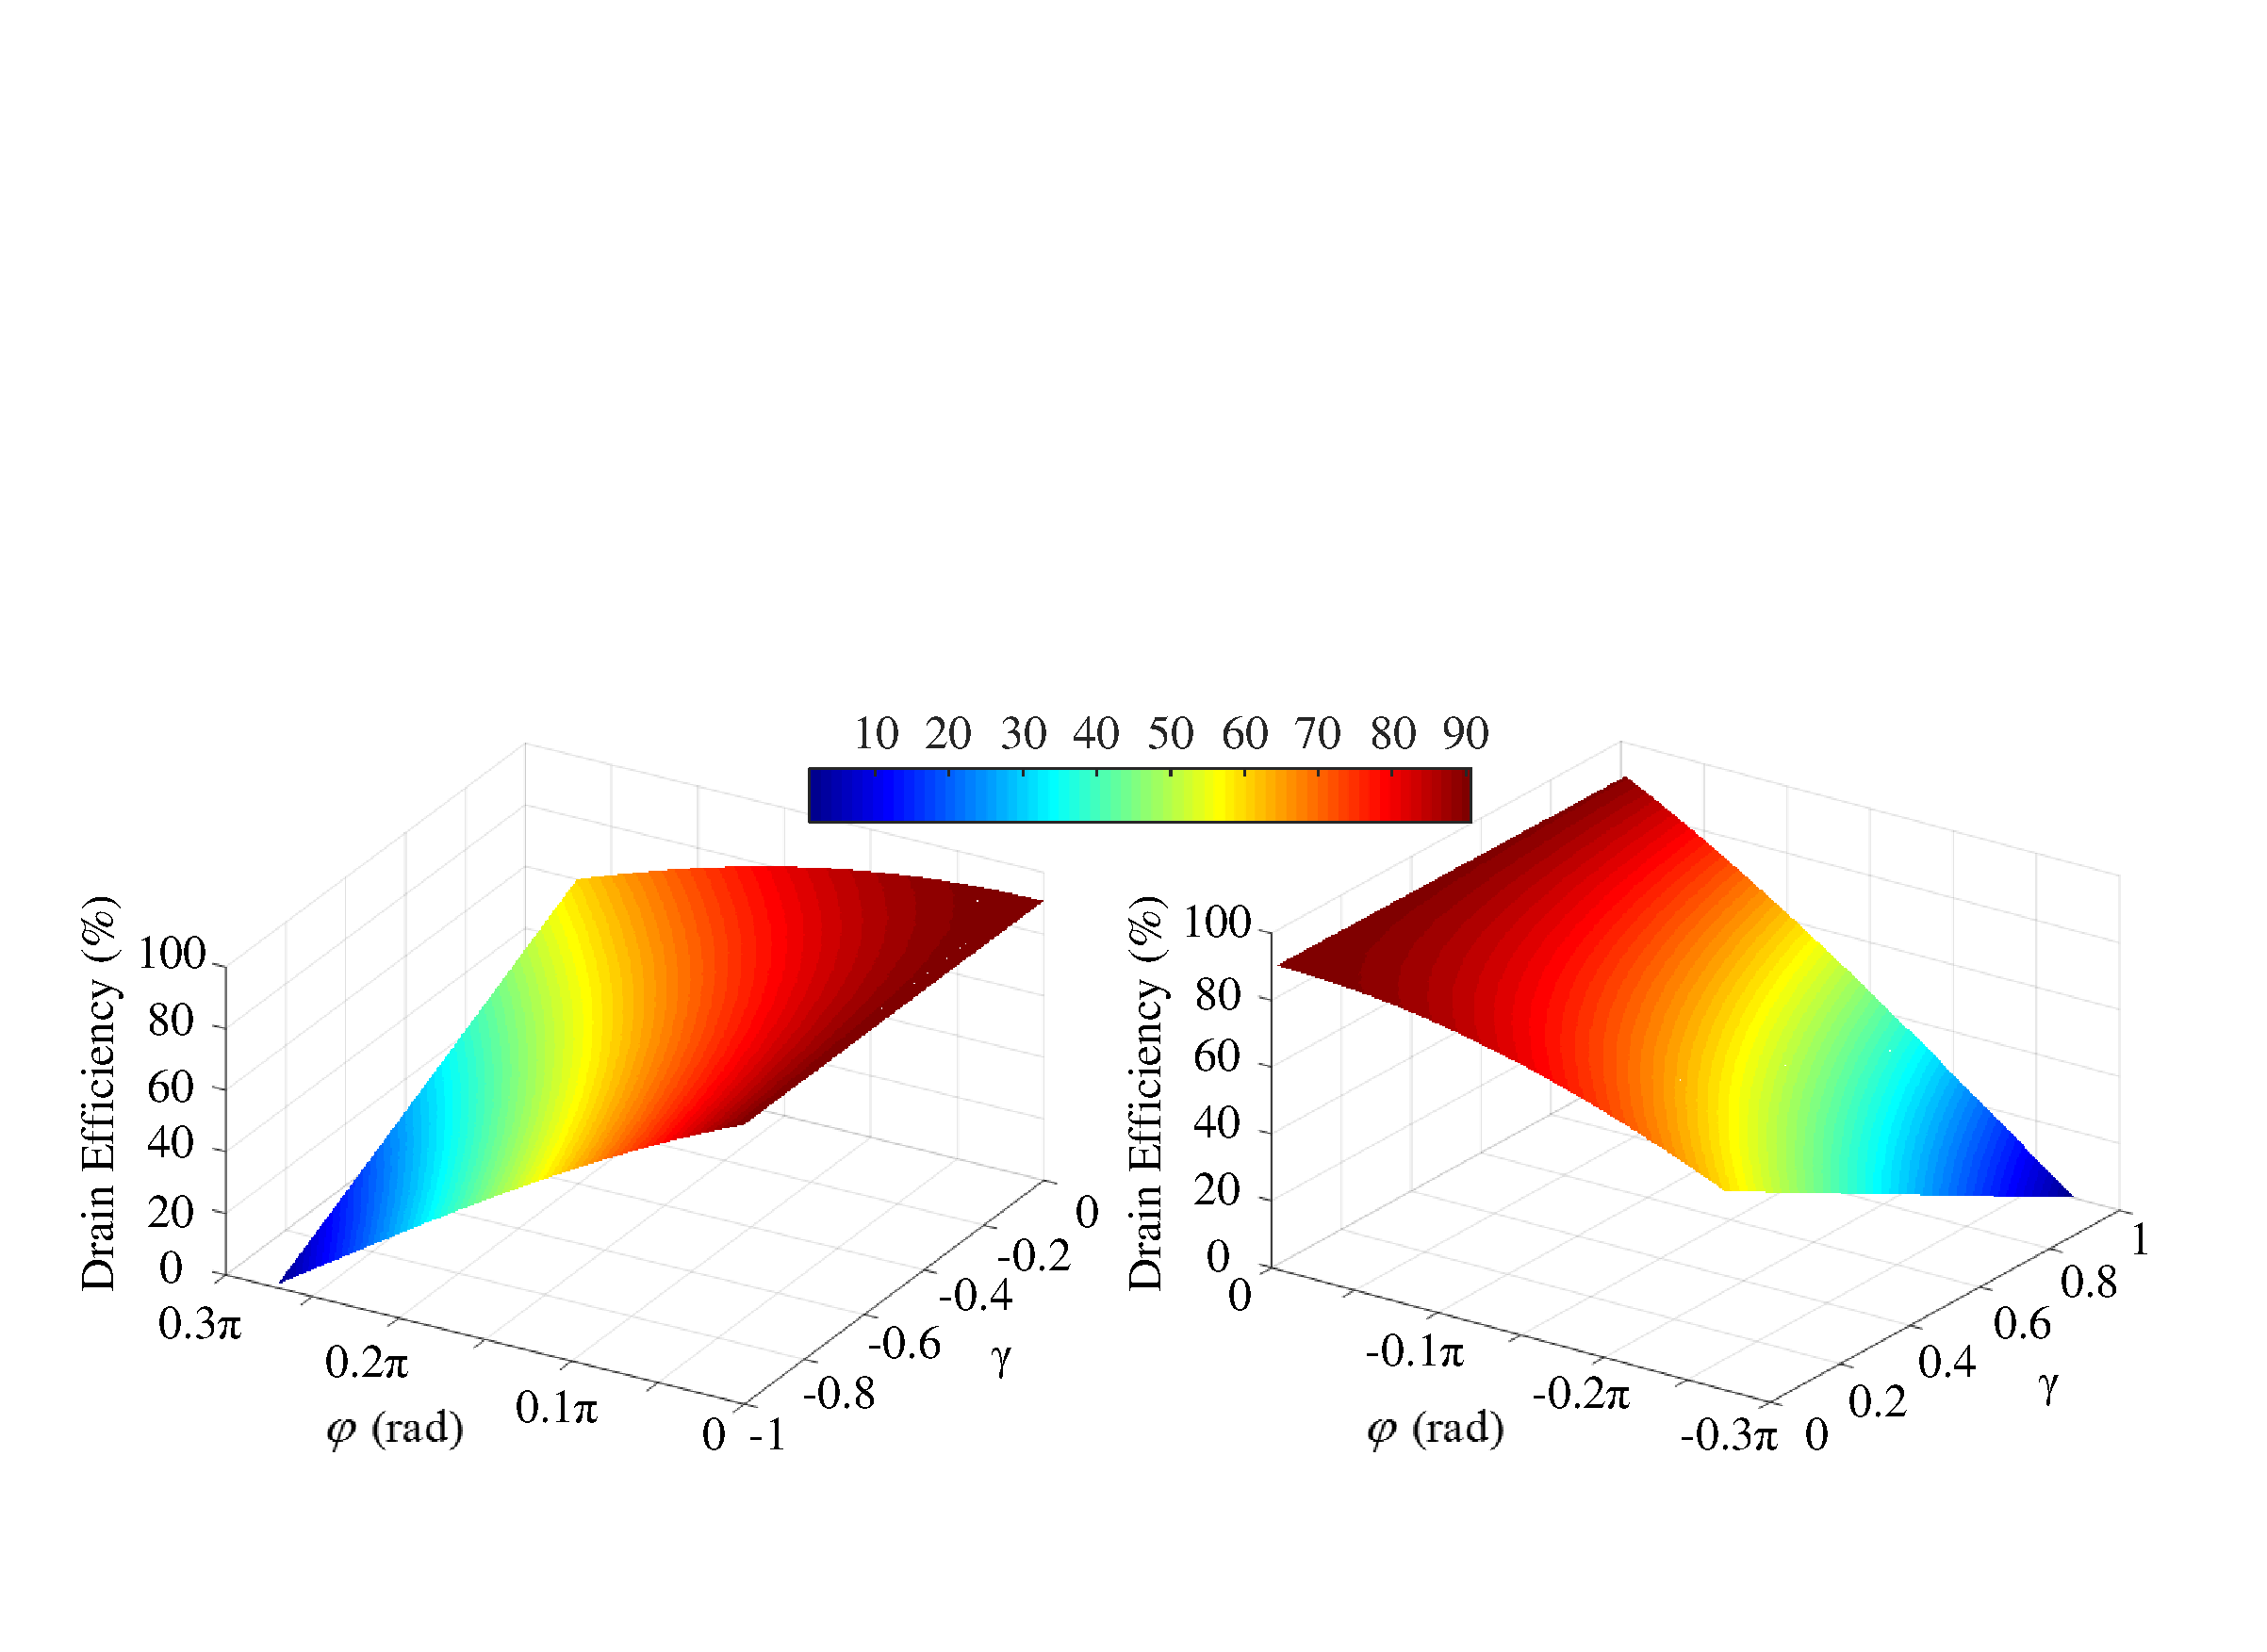
\includegraphics[width=12cm]{chapters/DE_CF.pdf}}
	\begin{itemize}[leftmargin=1.6cm,rightmargin=1.6cm]
		\item[\quad] \bicaption[\xiaosi 理论效率与$\gamma$和$\varphi$的关系]{\wuhao 理论效率与$\gamma$和$\varphi$的关系。 (a) $\alpha=1$; (b) $\alpha=2/\sqrt{3}$}{\wuhaob Theoretical DE versus $\gamma$ and $\varphi$. (a) $\alpha=1$; (b) $\alpha=2/\sqrt{3}$Theoretical DE versus $\gamma$ and $\varphi$. (a) $\alpha=1$; (b) $\alpha=2/\sqrt{3}$}
	\end{itemize}
\vspace{-1cm}


%\captionsetup{margin={1.6cm,1.6cm}}
%\bicaption[\xiaosi 理论效率与$\gamma$和$\varphi$的关系。]{\wuhao 理论效率与$\gamma$和$\varphi$的关系。 (a) $\alpha=1$; (b) $\alpha=2/\sqrt{3}$}{\wuhaob Theoretical DE versus $\gamma$ and $\varphi$. (a) $\alpha=1$; (b) $\alpha=2/\sqrt{3}$Theoretical DE versus $\gamma$ and $\varphi$. (a) $\alpha=1$; (b) $\alpha=2/\sqrt{3}$}


\end{figure}



\subsection{表}

表格格式参照写作指南。表格格式参照写作指南。表格格式参照写作指南。表格格式参照写作指南。表格格式参照写作指南。表格格式参照写作指南。表格格式参照写作指南。表格格式参照写作指南。表格格式参照写作指南。表格格式参照写作指南。表格格式参照写作指南。表格格式参照写作指南。表格格式参照写作指南。表格格式参照写作指南。表格格式参照写作指南。表格格式参照写作指南。

\vspace{0.1cm}

\begin{table}[h]
	\renewcommand{\arraystretch}{1.5}
	\centering
	\bicaption[\xiaosi 电流类型对效率的影响]{\wuhao 电流类型对效率的影响}{\wuhao Current type impact on efficiency}
	\begin{tabular}{p{3cm}p{3cm}p{3cm}p{3cm}}
		\toprule[1.5pt]
		\makecell[c]{\songti\wuhao 电流类型}&\makecell[c]{\songti\wuhao A}&\makecell[c]{\songti\wuhao B}&\makecell[c]{\songti\wuhao C}\\
		\hline
		\makecell[c]{\wuhao aaa}&\makecell[c]{\wuhao aa1}&\makecell[c]{\wuhao bb1}&\makecell[c]{\wuhao cc1}\\
		\bottomrule[1.5pt]
	\end{tabular}
   \label{tab:3.1} 	
\end{table}

表格格式参照写作指南。表格格式参照写作指南。表格格式参照写作指南。表格格式参照写作指南。表格格式参照写作指南。表格格式参照写作指南。表格格式参照写作指南。表格格式参照写作指南。表格格式参照写作指南。表格格式参照写作指南。表格格式参照写作指南。表格格式参照写作指南。表格格式参照写作指南。表格格式参照写作指南。表格格式参照写作指南。表格格式参照写作指南。

\vspace{-0.1cm}

\begin{table*}[h]
	\renewcommand{\arraystretch}{1.5}
	\bicaption[\xiaosi 高效率功放性能对比]{\wuhao 高效率功放性能对比}{\wuhao High-effiency power amplifier performance comparison}
	\label{tab_1}
	\centering
	\wuhao
	\begin{tabular}{c c c c c }
		\hline
		{\textbf{带宽}(GHz)}&{\textbf{功率}(dBm)}&{\textbf{效率}(\%)}&{\textbf{线性度}(dBc)}&{\textbf{信号带宽}(MHz)}\\
		\hline
		1.4--2.6&32--34&30--40 (DE)&-25 -- -30 (ACLR)&5\\
		\hline
		\multirow{2}{*}{2.1--2.7}&39&45 (DE) @ 2.14 GHz&--31 (ACLR)&\multirow{2}{*}{\diagbox{\qquad}{\qquad}}\\\cline{3-4}
		&(average)&40 (DE) @ 2.655 GHz&--30 (ACLR)& \\
		\hline
		3.5&38.1&59 (PAE)&30 (C/I)&5\\
		\hline
		\multirow{2}{*}{1.6--2.6}&36.0--38.5&45--60 (PAE)&30 (C/I)&5\\\cline{2-5}
		&35.3--37.5&40--55 (PAE)&--30 (ACLR)&20\\
		\hline
	\end{tabular}
\end{table*}

算法表示例:XXXXXXXX,如算法3-1所示。

\begin{table}[!htb]
	\setlength{\belowcaptionskip}{6pt}
	\setlength{\abovecaptionskip}{6pt}
	\centering
	%	\caption{\wuhao DQN算法训练过程}
	%	{\wuhao Table2-1 Training process of DQN\\[6pt]}
	\renewcommand{\arraystretch}{1.2}
	\begin{tabular}{p{13.2cm}}
		\toprule[1.5pt]
		\makecell[l]{\songti\wuhao 算法3-1 XXXXXX训练过程}\\
		\midrule[0.75pt]
		\makecell[l]{\wuhao 1: \ \ xxxxxx缓存$D$以及xxxxxx量为$\theta$的xxxxx络;}\\
		\makecell[l]{\wuhao 2: \ \ \textbf{for} episodes $=0, 1,\cdots ,E$ \textbf{do}}\\
		\makecell[l]{\wuhao 3: \quad \ \ 初始xxxxx向量$\Phi (s)$并将其作为xxxxxxxx值;}\\
		\makecell[l]{\wuhao 4: \quad \ \ \textbf{for} $t =0, 1,\cdots ,T$ \textbf{do}}\\
		\makecell[l]{\wuhao 5: \qquad \ \ 以xxx率$\epsilon$选xxxxx动作$a$;}\\
		\makecell[l]{\wuhao 6: \qquad \ \ 否xxx动作${{a}}={{\max }_{\hat{a}}}Q(\Phi ({{s}}),\hat{a}|\theta )$;}\\
		\makecell[l]{\wuhao 6: \qquad \ \ 执xxx动作$a$并观xxx奖励$r$和下一状态$s^{\prime }$;}\\
		\makecell[l]{\wuhao 7: \qquad \ \ 将经验$(\Phi ({{s}}),a,r,\Phi ({s^{\prime }}))$存储xxxx缓存$D$;}\\
		\makecell[l]{\wuhao 8: \qquad \ \ 从$D$中XXXX择$c$个样本$(\Phi ({{s_j}}),a_j,r_j,\Phi ({{s_j}^{\prime }}))$,并XXXXXXX计算$y_j$;
		}\\
		\makecell[l]{\wuhao 9: \qquad \ \ 根据xxxxx差;}\\
		\makecell[l]{\wuhao 10: \qquad xxxxxxx下降法更新$\theta$;}\\
		\makecell[l]{\wuhao 11: \quad \textbf{end for}}\\
		\makecell[l]{\wuhao 12: \textbf{end for}}\\
		\bottomrule[1.5pt]
	\end{tabular}
	\label{tab:2.1} 
\end{table}


\section{公式格式}

\begin{equation}
\left\{ \begin{aligned}
0.794 \le \zeta  \le 1 ~~~~~~~~~~~\\
0.631 \le \gamma  = \frac{{0.631}}{{{\zeta ^2}}} \le 1~~~~~~ \\
- \frac{1}{{2\gamma }} \le \delta  \le \frac{1}{{2\gamma }}~~~~~~~~~~~ \\
{Z_{c,low,f}} = 2{R_{opt}}(\gamma  + j\delta )~~~~~\\
{Z_{c,2f}} = {Z_{c,low,2f}} =  - j\frac{{3\pi }}{4}\gamma \delta {R_{opt}}
\end{aligned} \right.
\label{eq:3.1}
\end{equation}

\begin{equation}
\begin{aligned}
v(\theta ) = V_{DD}\cdot(1 - \alpha cos(\theta  + \varphi ) + \beta cos(3\theta  + 3\varphi ))\\
\cdot(1 - \gamma \sin (\theta  + \varphi )) ~~~~~- 1 \le \gamma  \le 1\
\end{aligned}
\label{eq:vd}
\end{equation}

\begin{equation}
\begin{aligned}
att\left( {{\bm{q}},{\bm{k}},{\bm{v}}} \right) = softmax\left( {\frac{{{\bm{qk}}^{\rm T} }}
	{{\sqrt {d_{\bm{k}} } }}} \right){\bm{v}}
\end{aligned}
\label{eq:2.12}
\end{equation}




\noindent
公式格式测试。${\mathbf{\Theta }} = \left\{ {{\theta _k}\left( n \right),\forall k,n} \right\}$

\section{印制要求}
涉密学位论文的印刷、制作、传递、存档等,须符合国家、学校相关保密要求。学位论文一律左侧装订。

中文摘要之前的前置部分(封面、中、英文题名页、独创性声明和使用授权书),采用单面印刷。

从中文摘要开始,采用双面印刷。

中文摘要及之后的前置部分,包括中文摘要、ABSTRACT、目录、图目录(如有)、表目录(如有)、主要符号表(如有)、缩略词表(如有),在双面印刷时,若某部分页数为奇数,则该部分最后一页单面印刷。例如:若“摘要”只有1页,则其页码是“Ⅰ”,第“Ⅰ”页纸的背面为空白(无页眉或页码);“ABSTRACT”用新的一张纸印刷,页码从“Ⅱ”开始。

从第1章第1页开始,至论文最后1页,所有页面均双面印刷。例如:若第1章的最后1页为第17页,则第2章的第1页在第17页的背面印刷,页码为“18”(页眉是“重庆邮电大学博士(硕士)学位论文”)。

一次性双面打印整本学位论文技巧:除用于打印的版本外,电子版论文中一律不得出现空白页。论文打印建议使用PDF格式。为方便一次性双面打印,有时可在单面印刷的部分(如封面、中、英文题名页、独创性声明和使用授权书),或者双面打印只有1页的某部分内容(如摘要、ABSTRACT等)后插入1页空白页,该空白页不编排页眉页码;论文中出现的页码应前后连续,不得中断。


\section{本章小结}
本章介绍了……

% 第4章


\chapter{总结与展望}
\thispagestyle{others}
\pagestyle{others}
\xiaosi

\section{主要结论}

本文主要……

\section{研究展望}

更深入的研究……

以下文字用于测试。

以下文字用于测试。

以下文字用于测试。

以下文字用于测试。

以下文字用于测试。

以下文字用于测试。

以下文字用于测试。

以下文字用于测试。

以下文字用于测试。

以下文字用于测试。

以下文字用于测试。

以下文字用于测试。

以下文字用于测试。

以下文字用于测试。

以下文字用于测试。

以下文字用于测试。

以下文字用于测试。

以下文字用于测试。

以下文字用于测试。

以下文字用于测试。

以下文字用于测试。

以下文字用于测试。

以下文字用于测试。

以下文字用于测试。

以下文字用于测试。

以下文字用于测试。

以下文字用于测试。

以下文字用于测试。




%如果要增加章节数请在此加项

\backmatter

%取消后续章节的页眉上的章节编号
\renewcommand{\chaptermark}[1]{\markboth{#1}{}}

%参考文献

%参考文献



\begin{thebibliography}{200}
\wuhao %设置参考文献字体大小
\linespread{1}\selectfont
\setlength{\itemsep}{-1.4ex} %缩小条目间行距
\thispagestyle{others}
\pagestyle{others}

\makeatletter
\renewcommand\@biblabel[1]{[#1]\hfill} %序号左对齐
\makeatother
\setlength{\labelsep}{0cm}


\bibitem{ref1}
中华人民共和国国家质量监督检验检疫总局,中国国家标准化管理委员会. 学位论文编写规则: GB/T 7713.1-2006[S]. 北京: 中国标准出版社, 2007: 17-20.

\bibitem{ref2}

中华人民共和国国家质量监督检验检疫总局,中国国家标准化管理委员会. 科技报告编写规则: GB/T 7713.1-2014[S]. 北京: 中国标准出版社, 2007.

\bibitem{ref3}
王晓琰, 殷建芳, 王晓峰, 等. 关于连续出版会议论文著录格式的探讨[J]. 学报编辑论丛, 2019: 162-165.

\bibitem{ref4}
WU D, YAN J, WANG H, et al. Social Attribute Aware Incentive Mechanism for Device-to-Device Video Distribution[J]. IEEE Transactions on Multimedia, 2017, 19(8): 1908-1920.

\bibitem{ref5}
BAERGAMASCO F, ALBARELLI A, COSMO L, et al. Adopting an Unconstrained Ray Model in Light-Field Cameras for 3D Shape Reconstruction[C]. IEEE Conference on Computer Vision and Pattern Recognition, Boston, USA, 2015: 3003-3012.

\bibitem{ref6}
竺可桢. 物理学[M]. 北京: 科学出版社, 1973, 56-60.

\bibitem{ref7}
国家技术监督局. 国际单位制及其应用: GB 3100-1993[S]. 北京: 中国标准出版社, 1994: 3-6.

\bibitem{ref8}
王晓琰, 殷建芳, 王晓峰, 等. 关于连续出版会议论文著录格式的探讨[J]. 学报编辑论丛, 2019: 162-165.

\bibitem{ref9}
WU D, YAN J, WANG H, et al. Social Attribute Aware Incentive Mechanism for Device-to-Device Video Distribution[J]. IEEE Transactions on Multimedia, 2017, 19(8): 1908-1920.

\bibitem{ref10}
BAERGAMASCO F, ALBARELLI A, COSMO L, et al. Adopting an Unconstrained Ray Model in Light-Field Cameras for 3D Shape Reconstruction[C]. IEEE Conference on Computer Vision and Pattern Recognition, Boston, USA, 2015: 3003-3012.

\bibitem{ref111}
国家技术监督局. 国际单位制及其应用: GB 3100-1993[S]. 北京: 中国标准出版社, 1994: 3-6.

\bibitem{ref11}
竺可桢. 物理学[M]. 北京: 科学出版社, 1973, 56-60.

\bibitem{ref12}
国家技术监督局. 国际单位制及其应用: GB 3100-1993[S]. 北京: 中国标准出版社, 1994: 3-6.

\bibitem{ref1122}
竺可桢. 物理学[M]. 北京: 科学出版社, 1973, 56-60.

\bibitem{ref1133}
竺可桢. 物理学[M]. 北京: 科学出版社, 1973, 56-60.

\bibitem{ref13}
BAERGAMASCO F, ALBARELLI A, COSMO L, et al. Adopting an Unconstrained Ray Model in Light-Field Cameras for 3D Shape Reconstruction[C]. IEEE Conference on Computer Vision and Pattern Recognition, Boston, USA, 2015: 3003-3012.

\bibitem{ref14}
BAERGAMASCO F, ALBARELLI A, COSMO L, et al. Adopting an Unconstrained Ray Model in Light-Field Cameras for 3D Shape Reconstruction[C]. IEEE Conference on Computer Vision and Pattern Recognition, Boston, USA, 2015: 3003-3012.

\bibitem{ref15}
BAERGAMASCO F, ALBARELLI A, COSMO L, et al. Adopting an Unconstrained Ray Model in Light-Field Cameras for 3D Shape Reconstruction[C]. IEEE Conference on Computer Vision and Pattern Recognition, Boston, USA, 2015: 3003-3012.

\bibitem{ref16}
BAERGAMASCO F, ALBARELLI A, COSMO L, et al. Adopting an Unconstrained Ray Model in Light-Field Cameras for 3D Shape Reconstruction[C]. IEEE Conference on Computer Vision and Pattern Recognition, Boston, USA, 2015: 3003-3012.

\bibitem{ref17}
BAERGAMASCO F, ALBARELLI A, COSMO L, et al. Adopting an Unconstrained Ray Model in Light-Field Cameras for 3D Shape Reconstruction[C]. IEEE Conference on Computer Vision and Pattern Recognition, Boston, USA, 2015: 3003-3012.


\end{thebibliography}

%\bibliographystyle{unsrt}
%%
%%
%%% 此参考文献名为ref.bib文件
%%
%\bibliography{ref}
%\thispagestyle{others}





\clearpage

%如果没有附录请自行删除以下页面

%附录A
%\specialsectioning
\chapter{附录A 各学院中英文名称对照表}
\thispagestyle{others}

\begin{table}[h]
	\renewcommand{\arraystretch}{1.5}
	\centering
	\begin{tabular}{p{2cm}p{3cm}p{8.5cm}}
		\toprule[1.5pt]
		\makecell[c]{\songti\xiaosi\bfseries 序号}&\makecell[l]{\songti\xiaosi\bfseries 中文名称}&\makecell[l]{\songti\xiaosi\bfseries 英文名称}\\
		\hline
		\makecell[c]{\wuhao 01}&\makecell[l]{\wuhao 通信工程学院}&\makecell[c]{\wuhao School of Communications and Information Engineering}\\
		\bottomrule[1.5pt]
	\end{tabular}
	
\end{table}

\clearpage

%附录B
%%\specialsectioning
\chapter{附录B 常见一级学科中英文名称对照表}
\thispagestyle{others}



\begin{table}[h]
	\renewcommand{\arraystretch}{1.5}
	\centering
	\begin{tabular}{p{2cm}p{3cm}p{8.5cm}}
		\toprule[1.5pt]
		\makecell[c]{\songti\xiaosi\bfseries 代码}&\makecell[l]{\songti\xiaosi\bfseries 中文名称}&\makecell[l]{\songti\xiaosi\bfseries 英文名称}\\
		\hline
		\makecell[c]{\wuhao 0810}&\makecell[l]{\wuhao 信息与通信工程}&\makecell[l]{\wuhao Information and Communication Engineering}\\
		\bottomrule[1.5pt]
	\end{tabular}
	
\end{table}

\clearpage

%附录C
%%\specialsectioning

\chapter{附录C 常见专业学位类别中英文名称对照表}

\thispagestyle{others}


\begin{table}[h]
	\renewcommand{\arraystretch}{1.5}
	\centering
	\begin{tabular}{p{2cm}p{3cm}p{8.5cm}}
		\toprule[1.5pt]
		\makecell[c]{\songti\xiaosi\bfseries 代码}&\makecell[l]{\songti\xiaosi\bfseries 中文名称}&\makecell[l]{\songti\xiaosi\bfseries 英文名称}\\
		\hline
		\makecell[c]{\wuhao 1256}&\makecell[l]{\wuhao 工程管理}&\makecell[l]{\wuhao Engineering Management}\\
		\bottomrule[1.5pt]
	\end{tabular}
	
\end{table}

\clearpage

%作者简介
\specialsectioning


\chapter{作者简介}
\thispagestyle{others}
\pagestyle{others}
\xiaosi

\section{1. \ 基本情况}
张某某,男,重庆人,1993年8月出生,重庆邮电大学XX学院XX专业2018级博士研究生。

\section{2. \ 教育和工作经历}

\section{3. \ 攻读学位期间的研究成果}

\vspace{0.2cm}

\subsection{3.1 \ 发表的学术论文和著作}


\subsection{3.2 \ 申请(授权)专利}

\subsection{3.3 \ 参与的科研项目及获奖}

以下文字用于测试。

以下文字用于测试。

以下文字用于测试。

以下文字用于测试。

以下文字用于测试。

以下文字用于测试。

以下文字用于测试。

以下文字用于测试。

以下文字用于测试。

以下文字用于测试。

以下文字用于测试。

以下文字用于测试。

以下文字用于测试。

以下文字用于测试。

以下文字用于测试。

以下文字用于测试。

以下文字用于测试。

以下文字用于测试。

以下文字用于测试。

以下文字用于测试。

以下文字用于测试。

以下文字用于测试。

以下文字用于测试。

以下文字用于测试。

以下文字用于测试。

以下文字用于测试。





% 致谢
% 致谢
%\specialsectioning
\chapter{致 \quad 谢}
\thispagestyle{others}
\pagestyle{others}
\xiaosi

感谢老师、同学们的关心、支持和帮助!

感谢老师、同学们的关心、支持和帮助!

感谢老师、同学们的关心、支持和帮助!

感谢老师、同学们的关心、支持和帮助!

感谢老师、同学们的关心、支持和帮助!

感谢老师、同学们的关心、支持和帮助!

感谢老师、同学们的关心、支持和帮助!

感谢老师、同学们的关心、支持和帮助!

感谢老师、同学们的关心、支持和帮助!

感谢老师、同学们的关心、支持和帮助!

感谢老师、同学们的关心、支持和帮助!

感谢老师、同学们的关心、支持和帮助!

感谢老师、同学们的关心、支持和帮助!

感谢老师、同学们的关心、支持和帮助!

感谢老师、同学们的关心、支持和帮助!

感谢老师、同学们的关心、支持和帮助!

感谢老师、同学们的关心、支持和帮助!

感谢老师、同学们的关心、支持和帮助!

感谢老师、同学们的关心、支持和帮助!

感谢老师、同学们的关心、支持和帮助!

感谢老师、同学们的关心、支持和帮助!

感谢老师、同学们的关心、支持和帮助!

感谢老师、同学们的关心、支持和帮助!

感谢老师、同学们的关心、支持和帮助!

感谢老师、同学们的关心、支持和帮助!

感谢老师、同学们的关心、支持和帮助!

感谢老师、同学们的关心、支持和帮助!

感谢老师、同学们的关心、支持和帮助!

感谢老师、同学们的关心、支持和帮助!

感谢老师、同学们的关心、支持和帮助!

感谢老师、同学们的关心、支持和帮助!

感谢老师、同学们的关心、支持和帮助!

感谢老师、同学们的关心、支持和帮助!

感谢老师、同学们的关心、支持和帮助!

感谢老师、同学们的关心、支持和帮助!

感谢老师、同学们的关心、支持和帮助!

感谢老师、同学们的关心、支持和帮助!

感谢老师、同学们的关心、支持和帮助!

感谢老师、同学们的关心、支持和帮助!

感谢老师、同学们的关心、支持和帮助!

感谢老师、同学们的关心、支持和帮助!

感谢老师、同学们的关心、支持和帮助!

感谢老师、同学们的关心、支持和帮助!







\end{document}